\documentclass[12pt, a4paper]{report}

% ---- layout ---------------------------------------------------------------
\usepackage[utf8]{inputenc}
\usepackage[T1]{fontenc}
\usepackage[american]{babel}
\usepackage[margin=1in, top=1in, left=1.1in, right=1in, bottom=1in]{geometry}
\usepackage{setspace}
\usepackage{titlesec}
\usepackage{fancyhdr}
\usepackage{emptypage}

% ---- tables & graphics ----------------------------------------------------
\usepackage{graphicx}
\usepackage{booktabs}
\usepackage{multirow}
\usepackage{array}
\usepackage{tabularx}
\usepackage{longtable}
\usepackage{adjustbox}
\usepackage{float}
\usepackage{pdflscape}
\usepackage{colortbl}
\usepackage[dvipsnames,table]{xcolor}

% ---- math -----------------------------------------------------------------
\usepackage{amsmath}
\usepackage{amssymb}
\usepackage{amsfonts}

% ---- captions, links, refs ------------------------------------------------
\usepackage{caption}
\usepackage{subcaption}
\usepackage[hidelinks]{hyperref}
\usepackage{url}
\usepackage[toc,page]{appendix}
\usepackage{tikz}
\usetikzlibrary{shapes.geometric,arrows.meta,positioning,fit,backgrounds,calc,trees}

% ---- code listings (no shell-escape needed; Overleaf-safe) ----------------
\usepackage{listings}
\definecolor{codegreen}{rgb}{0.0,0.5,0.0}
\definecolor{codegray}{rgb}{0.5,0.5,0.5}
\definecolor{codepurple}{rgb}{0.58,0.0,0.82}
\definecolor{backcolour}{rgb}{0.96,0.96,0.94}
\definecolor{keywordblue}{rgb}{0.0,0.0,0.7}
\lstdefinestyle{mystyle}{
    backgroundcolor=\color{backcolour},
    commentstyle=\color{codegreen},
    keywordstyle=\color{keywordblue}\bfseries,
    numberstyle=\tiny\color{codegray},
    stringstyle=\color{codepurple},
    basicstyle=\ttfamily\footnotesize,
    breakatwhitespace=false,
    breaklines=true,
    captionpos=b,
    keepspaces=true,
    numbers=left,
    numbersep=6pt,
    showspaces=false,
    showstringspaces=false,
    showtabs=false,
    frame=lines,
    tabsize=2
}
\lstset{style=mystyle}
% VHDL language flavour
\lstdefinelanguage{myvhdl}{
  morekeywords={library,use,entity,architecture,component,port,generic,is,begin,
    end,process,if,then,else,elsif,signal,in,out,inout,std_logic,std_logic_vector,
    natural,downto,to,when,others,for,generate,map,of,type,array,record,and,or,not,
    xor,nand,nor},
  sensitive=false,
  morecomment=[l]{--},
  morestring=[b]"
}
\lstdefinelanguage{mypython}{
  morekeywords={def,return,import,from,as,for,in,if,elif,else,while,with,try,except,
    class,None,True,False,and,or,not,is,lambda,yield,raise,continue,break,pass},
  sensitive=true,
  morecomment=[l]{\#},
  morestring=[b]",
  morestring=[b]'
}

% ---- caption style --------------------------------------------------------
\captionsetup{font=small,labelfont=bf,justification=centering}
\definecolor{headercolor}{RGB}{0,0,128}
\definecolor{rowcolor}{RGB}{235,235,255}

\titleformat{\chapter}[display]
  {\normalfont\huge\bfseries\color{headercolor}}{\chaptertitlename\ \thechapter}{16pt}{\Huge}
\titlespacing*{\chapter}{0pt}{0pt}{24pt}

\setlength{\headheight}{16pt}
\pagestyle{fancy}
\fancyhf{}
\fancyhead[L]{\nouppercase{\leftmark}}
\fancyhead[R]{\thepage}
\renewcommand{\headrulewidth}{0.4pt}
\renewcommand{\chaptermark}[1]{\markboth{\chaptername\ \thechapter.\ #1}{}}

\setlength{\parindent}{0pt}
\setlength{\parskip}{0.6em}
\setcounter{secnumdepth}{3}
\setcounter{tocdepth}{2}
\onehalfspacing

% ---- thesis metadata ------------------------------------------------------
\newcommand{\reporttitle}{Design-Space Exploration of Fault-Tolerance and In-Field Monitoring Techniques for the Klessydra RISC-V Vector Accelerator}
\newcommand{\reportname}{Tesi di Laurea Magistrale in Ingegneria Meccatronica}
\newcommand{\studentname}{Boulos Mansour}
\newcommand{\teachername}{Rodriguez Condia Josie Esteban (DAUIN) \\ Sonza Reorda Matteo (DAUIN) \\ Guerrero Balaguera Juan David \\ Vilar de Farias Gustavo}
\newcommand{\repourl}{https://github.com/BoulosMansour/klessydra}

\begin{document}
\pagenumbering{roman}

\begin{titlepage}
\newcommand{\HRule}{\rule{\linewidth}{0.5mm}}
\centering


\includegraphics[scale=0.7]{img/polito.png}\\[1cm]

\textsc{\LARGE Politecnico di Torino}\\[1.2cm]
\textsc{\Large Department of Electronics and Telecommunications}\\[0.4cm]
\textsc{\large Collegio di Ingegneria Informatica, del Cinema e Meccatronica}\\[0.4cm]
\textsc{Master's Degree in Mechatronic Engineering}\\[0.4cm]
\textsc{Academic Year 2025/2026}\\[0.8cm]

\HRule \\[0.4cm]
{
\huge{\bfseries{\reporttitle}}\\[0.5cm]
\large{\bfseries{\reportname}}
}\\[0.4cm]
\HRule \\[1.2cm]

\begin{minipage}[t]{0.38\textwidth}
\begin{flushleft} \large
\emph{Candidate:}\\[0.2cm]
\studentname
\end{flushleft}
\end{minipage}
\hfill
\begin{minipage}[t]{0.58\textwidth}
\begin{flushright}
{\large \emph{Supervisors:}} \\[0.2cm]
\teachername
\end{flushright}
\end{minipage}\\[1.5cm]

\vfill
{\small Source code and reproducibility materials: \href{\repourl}{\repourl}}\\[0.4cm]
{\large \today}

\end{titlepage}

\cleardoublepage

\chapter*{Abstract}
\addcontentsline{toc}{chapter}{Abstract}
\markboth{Abstract}{Abstract}

The growing deployment of RISC-V processors in safety- and mission-critical
domains --- automotive, aerospace, and edge artificial intelligence --- demands
hardware that can tolerate and detect faults induced by radiation, ageing, and
environmental stress. Vector accelerators, which dominate both the silicon area
and the computational workload of modern embedded cores, are particularly
exposed. This thesis investigates the design and characterization of
fault-tolerance and in-field monitoring mechanisms for the SIMD vector
accelerator of the Klessydra RISC-V architecture.

The work begins by re-engineering the originally monolithic VHDL accelerator
into a modular, hierarchical design in which each functional unit --- adders,
multipliers, shifters, comparators, and accumulator --- is cleanly isolated,
enabling fault-tolerance mechanisms to be inserted at fine granularity. On this
basis, reusable Dual Modular Redundancy (DMR), providing error detection through
an error flag, and Triple Modular Redundancy (TMR), providing error masking
through majority voting, are developed and applied both selectively to
individual functional units and globally to the complete accelerator. This
produces a family of hardened configurations spanning a wide range of
protection-versus-cost trade-offs.

To complement the structural redundancy with run-time observability, an
automated tool is developed that injects IEEE~1687 (IJTAG) sensors --- including
thermal and activity monitors --- directly into the VHDL hierarchy and generates
the corresponding Tessent scripts to build the on-chip IJTAG access network,
allowing in-field health monitoring without manual rewiring of the design.

All configurations are functionally verified through simulation and synthesized
across multiple technology nodes spanning a mature, a mainstream, and an
advanced process, yielding a comprehensive characterization of the area, power,
and timing overhead of each redundancy scheme at both the functional-unit and
the full-accelerator level. The results quantify the cost of protection ---
showing that duplication-based detection and triplication-based masking incur
consistent and predictable area and power penalties across nodes, while the
choice of which functional unit to harden dominates the overall cost --- and
provide design guidelines for selecting the appropriate fault-tolerance strategy
under given reliability and resource constraints. The study further shows that,
when an accelerator is already replicated for throughput, adding voting-based
redundancy comes at a comparatively small marginal cost. Overall, the proposed
flow demonstrates a reusable, automatable methodology for hardening RISC-V vector
accelerators against faults while keeping them observable in the field.

\cleardoublepage

\chapter*{Acknowledgements}
\addcontentsline{toc}{chapter}{Acknowledgements}
\markboth{Acknowledgements}{Acknowledgements}

I would like to express my sincere gratitude to my supervisor and to the
Klessydra research group for their guidance, for granting access to the
Klessydra source code and the synthesis tool flow, and for the many discussions
that shaped the direction of this work.

I am grateful to the Politecnico di Torino and to the Department of Electronics
and Telecommunications for providing the environment and the electronic design
automation infrastructure --- including the Design Compiler installation and the
process design kits used throughout the experimental campaign --- without which
this study would not have been possible.

Finally, I thank my family and friends for their constant support and
encouragement throughout my studies.

\vspace{2cm}
\begin{flushright}
\textit{Boulos Mansour}\\
\textit{Turin, 2026}
\end{flushright}

\cleardoublepage

\tableofcontents
\listoffigures
\listoftables
\cleardoublepage

\chapter*{List of Acronyms}
\addcontentsline{toc}{chapter}{List of Acronyms}
\markboth{List of Acronyms}{List of Acronyms}

\begin{longtable}{p{2.6cm} p{11cm}}
\toprule
\textbf{Acronym} & \textbf{Definition} \\
\midrule
\endhead
ALU      & Arithmetic Logic Unit \\
ASIC     & Application-Specific Integrated Circuit \\
BIST     & Built-In Self-Test \\
CMOS     & Complementary Metal-Oxide-Semiconductor \\
DC       & Design Compiler (Synopsys) \\
DfT      & Design-for-Test \\
DMR      & Dual Modular Redundancy \\
DSP      & Digital Signal Processor / the Klessydra accelerator unit \\
ECC      & Error-Correcting Code \\
EDA      & Electronic Design Automation \\
FIT      & Failures In Time \\
FU       & Functional Unit \\
HDL      & Hardware Description Language \\
ICL      & Instrument Connectivity Language \\
IJTAG    & Internal JTAG (IEEE~1687) \\
ISA      & Instruction Set Architecture \\
JTAG     & Joint Test Action Group (IEEE~1149.1) \\
PCS      & Procedural Description Language (PDL) \\
PDK      & Process Design Kit \\
PDL      & Procedural Description Language \\
RISC     & Reduced Instruction Set Computer \\
RTL      & Register-Transfer Level \\
SEE      & Single-Event Effect \\
SET      & Single-Event Transient \\
SEU      & Single-Event Upset \\
SIB      & Segment Insertion Bit \\
SIMD     & Single Instruction, Multiple Data \\
SoC      & System-on-Chip \\
SPM      & Scratchpad Memory \\
TAP      & Test Access Port \\
TDR      & Test Data Register \\
TMR      & Triple Modular Redundancy \\
TPS      & Thread Pool Size \\
VHDL     & VHSIC Hardware Description Language \\
\bottomrule
\end{longtable}

\cleardoublepage

\pagenumbering{arabic}

\chapter{Introduction}
\label{ch:intro}

\section{Motivation}

The open RISC-V instruction set architecture (ISA)~\cite{riscv-isa} has moved, in less than a
decade, from an academic teaching vehicle to a credible foundation for
commercial silicon. Its modular, royalty-free nature allows designers to tailor
a processor precisely to an application: a minimal microcontroller core for a
deeply embedded sensor node, or a richly extended core with custom accelerators
for signal processing and machine learning at the edge. This flexibility is
precisely what makes RISC-V attractive in domains where general-purpose
processors are either too power-hungry or too inflexible --- automotive
electronics, avionics and space payloads, industrial control, and battery-powered
edge artificial-intelligence (AI) devices.

These same domains, however, are also the domains in which \emph{dependability}
is not optional. A processor steering a vehicle, controlling an actuator, or
running a perception network must continue to produce correct results even in
the presence of transient and permanent faults. Such faults are no longer rare
curiosities confined to space applications. As CMOS technology has scaled into
the deep-nanometre regime, the electrical charge that distinguishes a logic
\texttt{1} from a logic \texttt{0} has shrunk dramatically, so that a single
energetic particle, a voltage glitch, or an ageing-induced threshold shift can
now flip a bit or momentarily corrupt a combinational result even at terrestrial
altitudes. Radiation-induced single-event effects (SEEs), supply-voltage noise,
electromigration, and bias-temperature instability all conspire to make modern
integrated circuits statistically more likely to err over their service life.

Within a modern embedded core, the \emph{vector accelerator} is a particularly
critical and particularly exposed component. Single-Instruction-Multiple-Data
(SIMD) accelerators exist precisely because they pack a large amount of
arithmetic into a small amount of control: wide datapaths of adders,
multipliers, shifters, and comparators that operate in lockstep on many data
elements at once. Consequently they tend to dominate both the silicon area and
the dynamic activity of the core. A fault that strikes the accelerator datapath
can silently corrupt every element of a vector result, and because the
accelerator is so heavily exercised, the probability that a fault is actually
\emph{activated} into an error is high. Protecting the vector accelerator is
therefore one of the highest-leverage decisions a designer can make when
hardening a RISC-V core for a critical application.

\section{The Klessydra vector accelerator}

This thesis works with the vector accelerator of \emph{Klessydra}, a family of
RISC-V cores developed for research into interleaved-multithreading and
SIMD acceleration. The Klessydra accelerator --- referred to throughout this
document as the \emph{DSP} unit --- implements a configurable SIMD datapath that
can be parameterised in its data width, the number of parallel SIMD lanes, the
size of the scratchpad memory, and the number of hardware threads it serves.
Internally it is organised around a small set of functional units: vector
adders, vector multipliers, vector shifters, vector comparators, and an
accumulation unit, fed by a mapping stage that distributes operands and gathers
results.

In its original form the accelerator was described as a largely monolithic block
of VHDL. While functionally complete, this structure is awkward for reliability
engineering: there is no clean boundary at which a redundancy mechanism can be
attached to, say, ``just the multiplier'' without disturbing the surrounding
logic. A central premise of this work is that \emph{fault tolerance is a
structural property as much as a functional one} --- to harden a design
selectively and to measure the cost of doing so, the design must first be
decomposed into well-defined, independently instantiable units.

\section{Problem statement}

Given the Klessydra vector accelerator, this thesis addresses three closely
related questions:

\begin{enumerate}
  \item \textbf{Structure.} How can the accelerator be re-engineered into a
        modular, hierarchical form in which each functional unit is cleanly
        isolated, so that redundancy can be inserted at arbitrary granularity ---
        from a single functional unit up to the entire accelerator?
  \item \textbf{Protection.} What reusable hardware redundancy mechanisms can be
        built on top of this modular structure, and what is the \emph{quantified
        cost} --- in area, power, and timing --- of applying them at different
        granularities and across different technology nodes?
  \item \textbf{Observability.} How can the hardened accelerator additionally be
        made \emph{observable in the field}, so that its health can be monitored
        at run time, and can this instrumentation be inserted automatically
        rather than by error-prone manual editing of the HDL?
\end{enumerate}

\section{Contributions}

In answering these questions, the thesis makes the following contributions.

\begin{itemize}
  \item \textbf{A modular re-engineering of the Klessydra DSP accelerator.}
        The monolithic datapath is restructured into a clean hierarchy in which
        adders, multipliers, shifters, comparators, and the accumulator are
        separate VHDL entities with explicit interfaces, multi-stage pipelined
        sub-blocks, and a mapping layer that is itself replication-aware.

  \item \textbf{Reusable DMR and TMR redundancy primitives.} Two small,
        technology-independent VHDL building blocks --- a Dual-Modular-Redundancy
        comparator with an error flag, and a Triple-Modular-Redundancy majority
        voter --- are designed and then wrapped around each functional unit and
        around the full accelerator, yielding a complete family of hardened
        configurations.

  \item \textbf{An automated IEEE~1687 (IJTAG) sensor-insertion tool.} A
        pragma-driven tool scans the VHDL hierarchy, inserts parameterisable
        on-chip sensors (activity and thermal monitors), and generates the
        Tessent scripts that extract the instrument connectivity and build the
        IJTAG access network with the necessary Segment Insertion Bits (SIBs),
        all without manual rewiring of the design.

  \item \textbf{A cross-node design-space exploration.} Every configuration is
        synthesised across three technology nodes spanning a mature, a
        mainstream, and an advanced process, and the resulting area, power, and
        timing data are reduced to a consistent set of comparisons, tables, and
        design guidelines.
\end{itemize}

\section{Thesis outline}

The remainder of this thesis is organised as follows.
Chapter~\ref{ch:background} reviews the technical background: the RISC-V ISA and
vector acceleration, the physics and modelling of faults in nanometre CMOS, the
classical redundancy techniques, and the IEEE~1149.1 / IEEE~1687 test and
monitoring standards.
Chapter~\ref{ch:architecture} describes the Klessydra DSP accelerator and the
modular re-engineering that underpins the rest of the work.
Chapter~\ref{ch:framework} presents the DMR and TMR fault-tolerance framework
and the two ways in which it is applied: per-functional-unit hardening and
replication-based redundancy.
Chapter~\ref{ch:ijtag} presents the automated IJTAG monitoring framework and the
sensor-insertion tool.
Chapter~\ref{ch:experiment} details the experimental setup: the synthesis flow,
the technology nodes, the configuration matrix, and the metrics.
Chapter~\ref{ch:results} reports and discusses the results of the design-space
exploration.
Chapter~\ref{ch:conclusion} concludes and outlines directions for future work.

\chapter{Background and Related Work}
\label{ch:background}

This chapter establishes the technical foundations on which the thesis builds.
Section~\ref{sec:riscv} introduces the RISC-V ISA and the rationale for vector
acceleration. Section~\ref{sec:faults} reviews the physical origins and the
abstract modelling of hardware faults. Section~\ref{sec:redundancy} surveys the
classical hardware redundancy techniques, focusing on the duplication- and
triplication-based schemes used in this work. Section~\ref{sec:ijtag-bg}
introduces the IEEE~1149.1 and IEEE~1687 standards for test and in-field
instrument access. Section~\ref{sec:related} positions the thesis with respect
to related work.

\section{RISC-V and vector acceleration}
\label{sec:riscv}

\subsection{The RISC-V instruction set architecture}

RISC-V~\cite{riscv-isa} is an open, royalty-free instruction set architecture organised as a
small mandatory base integer ISA (\texttt{RV32I} / \texttt{RV64I}) together with
a set of optional standard extensions --- integer multiplication and division
(\texttt{M}), atomics (\texttt{A}), single- and double-precision floating point
(\texttt{F}/\texttt{D}), compressed instructions (\texttt{C}), and the vector
extension (\texttt{V})~\cite{riscv-vector}, among others. Crucially, the ISA explicitly reserves
encoding space for \emph{non-standard, custom extensions}. This is what makes
RISC-V so attractive for domain-specific acceleration: a designer can add
application-specific instructions and the hardware to execute them, while
remaining within a coherent and well-documented architectural framework.

The openness of the ISA has a second consequence that is directly relevant to
this thesis. Because the architecture and many high-quality implementations are
open, researchers can modify the microarchitecture freely --- inserting
redundancy, instrumentation, or monitoring logic at any level of the hierarchy
--- something that is simply impossible with the closed, encrypted RTL of most
commercial cores.

\subsection{Data-level parallelism and SIMD accelerators}

A large fraction of the workloads that run on embedded and edge devices ---
digital filtering, fast transforms, linear algebra, and the convolutions at the
heart of neural networks --- are characterised by \emph{data-level parallelism}:
the same operation is applied independently to many data elements. The natural
hardware answer is the Single-Instruction-Multiple-Data (SIMD) paradigm, in
which one instruction drives a wide datapath that processes many elements
simultaneously.

A SIMD vector accelerator amortises the cost of instruction fetch, decode, and
control over a large amount of arithmetic, which is why such accelerators
deliver excellent energy efficiency on suitable workloads. The flip side, and
the reason this thesis focuses on them, is that the resulting wide arithmetic
datapath --- arrays of adders, multipliers, shifters, and comparators ---
typically dominates the area and the switching activity of the core. From a
reliability standpoint the accelerator is therefore both the \emph{largest}
target a fault can strike and the \emph{busiest}, so faults are activated into
errors with high probability.

\subsection{The Klessydra cores}

Klessydra~\cite{klessydra,klessydra-dsp} is a family of RISC-V cores designed around interleaved hardware
multithreading and configurable SIMD acceleration, intended for research and for
embedded use. The cores implement the RISC-V base ISA together with custom
vector instructions that are executed by a dedicated coprocessor, the DSP unit
studied here. Key configuration parameters --- the SIMD width, the number of
parallel accelerator lanes, the scratchpad-memory size, the data width, and the
thread-pool size --- are exposed as VHDL generics and package constants, so that
a single source base can be elaborated into a wide range of design points. This
parameterisation is exploited heavily in the present work: the same accelerator
source is synthesised under many different redundancy and replication settings.

\section{Faults, errors, and failures}
\label{sec:faults}

\subsection{Terminology}

It is useful to distinguish three levels following the classical dependability~\cite{avizienis}
taxonomy. A \emph{fault} is the physical or logical defect --- a flipped storage
bit, a stuck-at node, a momentary voltage glitch. An \emph{error} is the
manifestation of a fault in the system state --- an incorrect value held in a
register or propagating along a wire. A \emph{failure} occurs when an error
propagates to the system output and the delivered service deviates from the
specification. Fault tolerance is the art of breaking the chain from fault to
failure: either by \emph{detecting} an error before it becomes a failure, or by
\emph{masking} it so that it never reaches the output.

\subsection{Physical origins}

Several physical mechanisms produce faults in modern integrated circuits:

\begin{itemize}
  \item \textbf{Radiation-induced single-event effects (SEEs).} An energetic
        particle --- a cosmic-ray secondary neutron at terrestrial altitude, or
        a heavy ion in space --- deposits charge as it traverses the silicon. If
        the collected charge exceeds a node's critical charge $Q_{crit}$, the
        node's logic value is disturbed. When this disturbance flips a storage
        element it is a \emph{single-event upset} (SEU)\footnote{See~\cite{baumann} for a survey of radiation-induced soft errors in advanced technologies.}; when it produces a
        transient pulse in combinational logic that may be latched downstream it
        is a \emph{single-event transient} (SET).
  \item \textbf{Supply and timing noise.} Voltage droop, ground bounce, and
        crosstalk can momentarily corrupt logic values or cause a path to miss
        its timing, producing transient errors that are strongly workload- and
        environment-dependent.
  \item \textbf{Ageing and wear-out.} Bias-temperature instability,
        hot-carrier injection, and electromigration slowly shift device
        parameters over the service life, eventually turning marginal paths into
        permanent timing failures or open/short defects.
\end{itemize}

As $Q_{crit}$ falls with each technology generation, the susceptibility of an
individual node to transient upset tends to rise, even as the smaller node also
presents a smaller cross-section to an incident particle. The net effect is that
soft errors are a first-order reliability concern across the whole range of
technology nodes considered in this thesis.

\subsection{Fault models}

For design and verification purposes the physical mechanisms above are abstracted
into \emph{fault models}. The \emph{stuck-at} model, in which a node is
permanently fixed at \texttt{0} or \texttt{1}, underpins most manufacturing
test. The \emph{single-event-upset} model, a transient bit-flip of a storage
element, is the workhorse for soft-error analysis. \emph{Transition} and
\emph{path-delay} models capture timing-related and ageing faults. The
redundancy mechanisms developed in this thesis are agnostic to the precise model:
DMR detects any discrepancy between two copies, and TMR masks any single faulty
copy, regardless of whether the underlying cause was a particle strike, a glitch,
or a wear-out defect that has manifested in only one replica.

\section{Hardware redundancy techniques}
\label{sec:redundancy}

Fault tolerance is achieved by adding \emph{redundancy} --- in hardware, in
time~\cite{nicolaidis}, or in information. This thesis concentrates on \emph{spatial (hardware)
redundancy}, the dominant choice for protecting high-throughput datapaths where
re-execution in time would be too costly.

\subsection{Information redundancy}

Information redundancy adds check bits to data so that errors can be detected or
corrected. Parity detects single-bit errors; single-error-correcting,
double-error-detecting (SEC-DED) Hamming codes~\cite{ecc-hamming} are the standard protection for
memories and register files. Information redundancy is extremely efficient for
\emph{storage}, but it is awkward for arbitrary \emph{combinational arithmetic}:
protecting a multiplier with an arithmetic residue code, for instance, requires
a bespoke checker and does not generalise across functional units. For this
reason information codes are complementary to, rather than a replacement for, the
modular redundancy studied here.

\subsection{Dual Modular Redundancy (DMR)}

Dual Modular Redundancy duplicates a module and compares the two outputs
bit-by-bit. If the copies agree, the result is forwarded and no error is
flagged; if they disagree, an error flag is raised. DMR therefore provides
\emph{error detection} but not correction: it cannot, on its own, decide which of
the two copies is correct. Its appeal is its low cost --- roughly twice the logic
of the protected module plus a thin comparison layer --- and its generality: the
same comparator works for any module, regardless of its internal function. In a
system context the DMR error flag can trigger a recovery action such as
re-execution, rollback, or a transition to a safe state.

\subsection{Triple Modular Redundancy (TMR)}

Triple Modular Redundancy~\cite{vonneumann,koren} triplicates a module and feeds the three outputs into a
bitwise majority voter, whose output equals the value produced by at least two of
the three copies. As long as no more than one copy is faulty at any given bit,
the voter \emph{masks} the fault completely: the error never reaches the output
and no recovery action is required. The logic function of a single-bit
three-input majority voter is
\begin{equation}
  v = (a \wedge b) \vee (b \wedge c) \vee (a \wedge c),
  \label{eq:majority}
\end{equation}
where $a$, $b$, $c$ are the three replica outputs. TMR is the canonical choice
for systems that must continue operating correctly through a fault without
interruption, at the cost of roughly three times the logic of the protected
module plus the voter. The voter itself is a single point of failure and in the
most demanding applications is itself triplicated; in this work a single voter
per output bit is used, which is the common practice at the datapath level.

\subsection{Granularity and the cost of protection}

A key design decision --- and a central theme of this thesis --- is the
\emph{granularity} at which redundancy is applied. Redundancy can wrap a single
functional unit, a group of units, or an entire accelerator. Finer granularity
allows the designer to spend the area budget where it matters most (for example,
protecting only the multiplier, which is both large and arithmetically
intricate), while coarser granularity is simpler to deploy and protects more of
the design. Because the functional units differ enormously in size, the cost of
protection depends strongly on \emph{which} unit is hardened, not only on
\emph{whether} DMR or TMR is used --- a point that the experimental results in
Chapter~\ref{ch:results} make quantitatively explicit.

\subsection{Replication for throughput versus replication for reliability}

There is an important and often overlooked interaction between redundancy and
\emph{performance} replication. A SIMD accelerator may already instantiate
multiple parallel lanes to increase throughput. When such replication is already
present, the incremental cost of \emph{also} using those lanes for reliability
--- comparing or voting their results --- can be far smaller than building
redundancy from scratch, because the expensive datapath copies already exist.
This thesis evaluates both regimes: building redundancy around a single-lane
accelerator (Scenario~A), and adding voting on top of an already-replicated
multi-lane accelerator (Scenario~B).

\section{Test and in-field monitoring: JTAG and IJTAG}
\label{sec:ijtag-bg}

\subsection{IEEE 1149.1 (JTAG)}

The IEEE~1149.1 standard~\cite{jtag}, universally known as JTAG, defines a Test Access Port
(TAP) and boundary-scan architecture originally created to test the
interconnections of boards after assembly. A four- or five-wire serial interface
(\texttt{TCK}, \texttt{TMS}, \texttt{TDI}, \texttt{TDO}, and optionally
\texttt{TRST}) drives a finite-state machine that shifts data through scan
registers. Over time JTAG became the de-facto standard not just for boundary
scan but for debug access and on-chip instrument control.

\subsection{IEEE 1687 (IJTAG)}

As chips accumulated more and more embedded instruments --- built-in self-test
controllers, sensors, trimming and configuration registers --- the flat,
fixed JTAG data-register structure became unwieldy. IEEE~1687, or
\emph{Internal JTAG} (IJTAG), standardises~\cite{ijtag} a \emph{reconfigurable, hierarchical}
network for accessing these embedded instruments. Its central element is the
\emph{Segment Insertion Bit} (SIB), a small controllable element that can switch
a segment of the scan path --- and the instruments on it --- into or out of the
active chain. By nesting SIBs, the access network can be reconfigured on the fly
so that only the instruments of interest are included in the scan path, keeping
access times short even when hundreds of instruments are present.

IJTAG is accompanied by two description languages: the \emph{Instrument
Connectivity Language} (ICL), which describes the structure of the network and
the instruments, and the \emph{Procedural Description Language} (PDL), which
describes how to operate them. Commercial tools --- in this work, Siemens~\cite{tessent}
Tessent --- consume ICL to automatically synthesise the network hardware~\cite{ijtag-network} and the
retargetable access patterns.

\subsection{From manufacturing test to in-field monitoring}

Although born for manufacturing test, the IJTAG network is equally a vehicle for
\emph{in-field monitoring}. Embedded sensors --- thermal monitors, voltage and
activity sensors, ageing monitors --- can be attached to the IJTAG network as
instruments, and their readings retrieved at run time through the same standard
interface. This makes IJTAG a natural complement to the structural redundancy of
DMR and TMR: redundancy keeps the design \emph{correct} in the presence of
faults, while IJTAG-attached sensors keep it \emph{observable}, allowing a system
to track temperature, activity, and degradation over its service life. Combining
the two on the same accelerator is one of the goals of this thesis.

\section{Related work}
\label{sec:related}

Hardware redundancy for processors and accelerators is a mature field. TMR has
been used for decades in aerospace and space-grade designs, and lockstep
dual-core arrangements (a coarse form of DMR with comparison) are standard in
automotive safety microcontrollers~\cite{lockstep}. Reliable-systems design is treated comprehensively in~\cite{siewiorek,koren}. At finer granularity, selective hardening
--- protecting only the most vulnerable or most critical sub-blocks --- has been
explored extensively as a way to trade reliability against area and power, often
guided by fault-injection campaigns that rank sub-blocks by their contribution
to the overall failure rate~\cite{mukherjee,riscv-hardening}.

For RISC-V specifically, a growing body of work applies these techniques to open
cores: lockstep and TMR variants of small cores, ECC-protected register files
and memories~\cite{tmr-fpga}, and selectively hardened execution units. Vector and SIMD
accelerators, however, have received comparatively less attention despite their
outsized contribution to area and activity, and systematic, \emph{cross-node}
cost characterisations at the granularity of individual functional units are
scarce.

On the monitoring side, IEEE~1687 has been studied primarily as a test-access
mechanism, with more recent work using it to retarget access to in-field sensors
and BIST engines. The automated insertion of sensors into an HDL hierarchy,
coupled with automatic generation of the IJTAG network, is comparatively
under-explored, particularly in combination with structural redundancy on the
same design.

This thesis contributes to both strands by treating a single, parameterised
RISC-V vector accelerator as a common substrate on which (i) DMR and TMR are
applied at controllable granularity and characterised consistently across three
technology nodes, and (ii) an automated IJTAG sensor-insertion flow provides
in-field observability --- bringing reliability and monitoring together in one
reusable methodology.

\chapter{The Klessydra DSP Accelerator and its Modular Re-engineering}
\label{ch:architecture}

This chapter describes the vector accelerator that is the subject of the thesis
and the structural re-engineering that makes the rest of the work possible.
Section~\ref{sec:arch-overview} gives an overview of the accelerator and its
place in the Klessydra core. Section~\ref{sec:arch-datapath} walks through the
datapath and its functional units. Section~\ref{sec:arch-mapping} describes the
mapping and control layers and the replication mechanism.
Section~\ref{sec:arch-breakdown} explains the modular ``break-down'' of the
original monolithic design and why it is a prerequisite for selective hardening.

\section{Overview of the accelerator}
\label{sec:arch-overview}

The Klessydra DSP unit is a SIMD vector coprocessor attached to the Klessydra
RISC-V core. It executes custom vector instructions --- vector add, multiply,
shift, compare, and multiply-accumulate among them --- on operands held in a
dedicated scratchpad memory (SPM). The accelerator is deeply parameterised
through VHDL generics and package constants; the parameters most relevant to
this work are summarised in Table~\ref{tab:params}.

\begin{table}[htbp]
\centering
\caption{Principal configuration parameters of the Klessydra DSP accelerator,
with the values used as the experimental baseline in this thesis.}
\label{tab:params}
\small
\begin{tabular}{lp{8.2cm}c}
\toprule
Parameter & Meaning & Baseline value \\
\midrule
\texttt{Data\_Width}      & Scalar element width in bits                              & 32 \\
\texttt{SIMD}             & Number of SIMD sub-lanes per accelerator lane             & 2 \\
\texttt{SIMD\_Width}      & Aggregate datapath width (\texttt{SIMD}$\times$32) in bits & 64 \\
\texttt{ACCL\_NUM}        & Number of parallel accelerator lanes                      & 1 / 3 \\
\texttt{FU\_NUM}          & Number of functional-unit sets                            & 1 / 3 \\
\texttt{THREAD\_POOL\_SIZE} & Number of interleaved hardware threads                  & 3 \\
\texttt{SPM\_NUM}         & Number of scratchpad banks                                & 4 \\
\texttt{replicate\_accl\_en} & Enables the replicated multi-lane datapath             & 0 / 1 \\
\bottomrule
\end{tabular}
\end{table}

When \texttt{replicate\_accl\_en} is disabled, a single accelerator lane
(\texttt{ACCL\_NUM}~$=$~\texttt{FU\_NUM}~$=$~1) serves the thread pool; this is
the substrate for per-functional-unit hardening (Scenario~A in
Chapter~\ref{ch:framework}). When replication is enabled, three lanes are
instantiated (\texttt{ACCL\_NUM}~$=$~\texttt{FU\_NUM}~$=$~3), which is the
substrate for replication-based redundancy (Scenario~B).

\section{The datapath and its functional units}
\label{sec:arch-datapath}

The heart of the accelerator is its arithmetic datapath, organised as a set of
pipelined functional units (FUs) fed by an input mapping stage and drained by an
output mapping stage. Figure~\ref{fig:datapath} sketches the structure.

\begin{figure}[htbp]
\centering
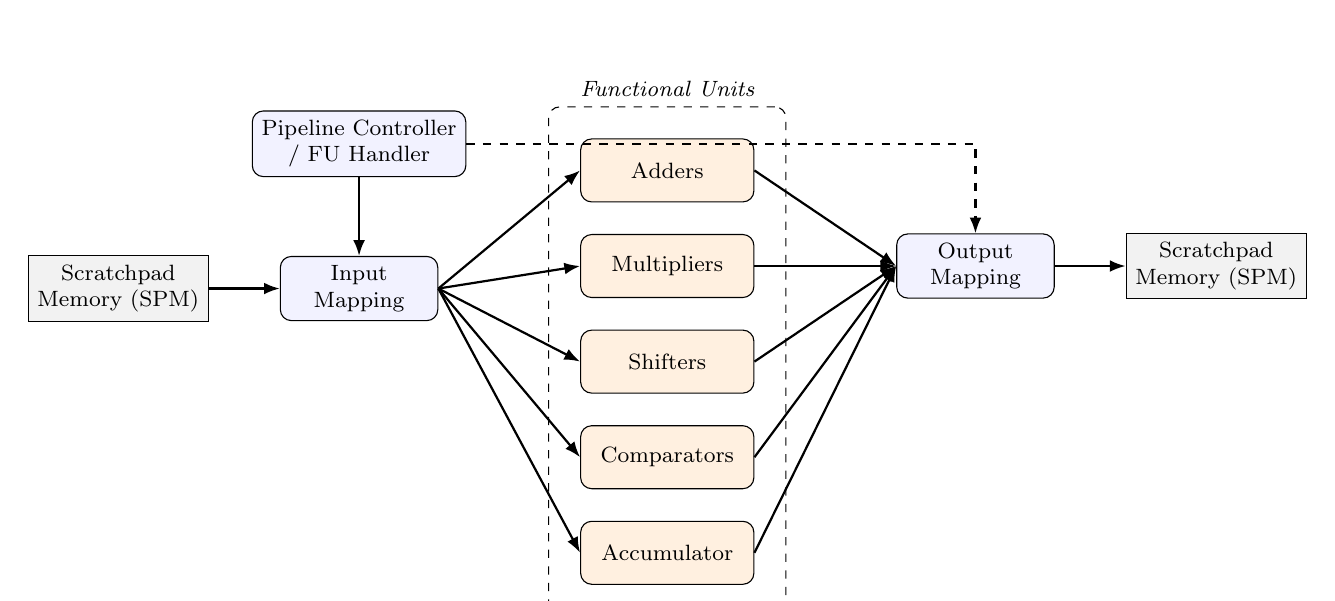
\begin{tikzpicture}[
  node distance=6mm and 9mm,
  box/.style={draw, rounded corners, minimum height=8mm, minimum width=20mm, align=center, font=\footnotesize, fill=blue!5},
  fu/.style={draw, rounded corners, minimum height=8mm, minimum width=22mm, align=center, font=\footnotesize, fill=orange!12},
  io/.style={draw, minimum height=8mm, minimum width=18mm, align=center, font=\footnotesize, fill=gray!10},
  arr/.style={-{Latex[length=2mm]}, thick}
]
\node[io] (spm) {Scratchpad\\Memory (SPM)};
\node[box, right=of spm] (inmap) {Input\\Mapping};
\node[fu, right=18mm of inmap, yshift=15mm] (add) {Adders};
\node[fu, below=4mm of add] (mul) {Multipliers};
\node[fu, below=4mm of mul] (shf) {Shifters};
\node[fu, below=4mm of shf] (cmp) {Comparators};
\node[fu, below=4mm of cmp] (acc) {Accumulator};
\node[box, right=18mm of mul] (outmap) {Output\\Mapping};
\node[io, right=of outmap] (spm2) {Scratchpad\\Memory (SPM)};
\node[box, above=10mm of inmap] (ctrl) {Pipeline Controller\\/ FU Handler};

\draw[arr] (spm) -- (inmap);
\foreach \f in {add,mul,shf,cmp,acc} \draw[arr] (inmap.east) -- (\f.west);
\foreach \f in {add,mul,shf,cmp,acc} \draw[arr] (\f.east) -- (outmap.west);
\draw[arr] (outmap) -- (spm2);
\draw[arr] (ctrl.south) -- (inmap.north);
\draw[arr, dashed] (ctrl.east) -| (outmap.north);
\begin{scope}[on background layer]
\node[draw, dashed, rounded corners, fit=(add)(mul)(shf)(cmp)(acc), inner sep=4mm, label={[font=\footnotesize\itshape]above:Functional Units}] {};
\end{scope}
\end{tikzpicture}
\caption{Block-level structure of the Klessydra DSP accelerator. Operands are
read from the scratchpad memory, distributed by the input mapping stage to the
functional units, and the results are gathered by the output mapping stage and
written back. The pipeline controller and FU handler sequence the units.}
\label{fig:datapath}
\end{figure}

\subsection{Vector adders}

The adder unit performs vector additions and subtractions and is configurable in
the way it propagates carries, so that one physical adder array can implement
byte-wise (\texttt{KADDV8}), half-word (\texttt{KADDV16}), or full-word
(\texttt{KADDV32}) additions by selectively breaking or passing the carry chain.
Internally it is pipelined across two stages (\texttt{DSP\_Adders\_stg\_1} and
\texttt{DSP\_Adders\_stg\_2}) with a synchronisation block
(\texttt{DSP\_Adders\_Sync}) that aligns results to the pipeline. The adder also
exports the most-significant-bit information used by the comparator unit.

\subsection{Vector multipliers}

The multiplier unit is the largest and most arithmetically complex functional
unit. It is built as a multi-stage pipeline
(\texttt{DSP\_Multipliers\_stg\_1}, a combinational partial-product stage
\texttt{DSP\_Multipliers\_stg\_1\_comb}, and \texttt{DSP\_Multipliers\_stg\_2})
so that the long multiplication critical path is broken into balanced pipeline
stages. Because of its size, the multiplier dominates the area cost of any
redundancy scheme that includes it --- a fact that the results in
Chapter~\ref{ch:results} make very visible.

\subsection{Vector shifters}

The shifter unit performs logical and arithmetic shifts across the vector lanes.
It comprises a combinational shift network (\texttt{DSP\_Shifters\_comb}) and two
pipeline stages (\texttt{DSP\_Shifters\_stg\_1}, \texttt{DSP\_Shifters\_stg\_2}).
Its area is modest and comparable to the adder.

\subsection{Vector comparators}

The comparator unit (\texttt{DSP\_Comparators\_Unit}) evaluates relational
operations across the vector elements, consuming the most-significant-bit
information exported by the adder. It is the smallest of the four arithmetic
functional units, which makes it the cheapest to protect.

\subsection{Accumulator}

The accumulation stage (\texttt{RTL-Accumulator}) implements the reduction
required by multiply-accumulate-style instructions, summing partial results
across iterations. In the present study the accumulator is treated as part of
the surrounding datapath rather than hardened individually, but the modular
structure would allow it to be wrapped just like the other units.

\section{Mapping, control, and replication}
\label{sec:arch-mapping}

\subsection{Mapping stages}

The \texttt{DSP\_Mapping} layer is responsible for routing operands from the
scratchpad to the functional units and routing results back. It exists in two
flavours --- a \emph{multithread} mapper
(\texttt{DSP\_Mapping\_IN\_Unit\_Multithread} and the matching out-mapper) and a
\emph{multicore} mapper (\texttt{DSP\_Mapping\_IN\_Unit\_Multicore} and
\texttt{DSP\_Mapping\_Multicore\_Out\_Mapper}). The multicore mapper is the one
exercised when the accelerator is replicated into multiple lanes, and, as
explained in Chapter~\ref{ch:framework}, it is also where replication-based
voting is inserted.

\subsection{Control: pipeline controller and FU handler}

Two control blocks sequence the datapath. The \texttt{DSP\_Pipeline\_Controller}
generates the stage-enable and halt signals that advance operands through the
functional-unit pipelines. The \texttt{DSP\_FU\_Handler} --- with dedicated
multicore (\texttt{MC}) and multithread (\texttt{MT}) variants and an enabler
synchroniser (\texttt{DSP\_FU\_Enabler\_Sync}) --- arbitrates which functional
unit is active for which thread or lane at any cycle, enabling the interleaved
multithreading that is characteristic of Klessydra. An exception-control unit
(\texttt{DSP\_Excpt\_Cntrl\_unit}) handles state recovery.

\subsection{Replication}

The top-level \texttt{replicate\_accl\_en} generic switches the accelerator
between a single-lane and a three-lane configuration. In the replicated
configuration three complete accelerator lanes operate in parallel, multiplying
throughput. This replicated datapath is significant for reliability because the
expensive functional-unit copies it instantiates can be \emph{reused} for
redundancy: rather than building new replicas, the redundancy logic simply
compares or votes the results that the lanes already produce. The cost of doing
so is quantified in Chapter~\ref{ch:results}.

\section{The modular break-down}
\label{sec:arch-breakdown}

\subsection{From monolith to hierarchy}

In its original form, much of the accelerator's arithmetic was expressed as a
single, tightly interwoven block. While this is acceptable for a fixed design,
it is hostile to reliability engineering: there is no entity boundary at which a
redundancy wrapper can be attached to one functional unit without entangling it
with the others, and there is no clean place to insert instrumentation. The
first engineering task of this thesis was therefore to \emph{break down} the
accelerator into the clean hierarchy summarised in Figure~\ref{fig:hierarchy}.

\begin{figure}[htbp]
\centering
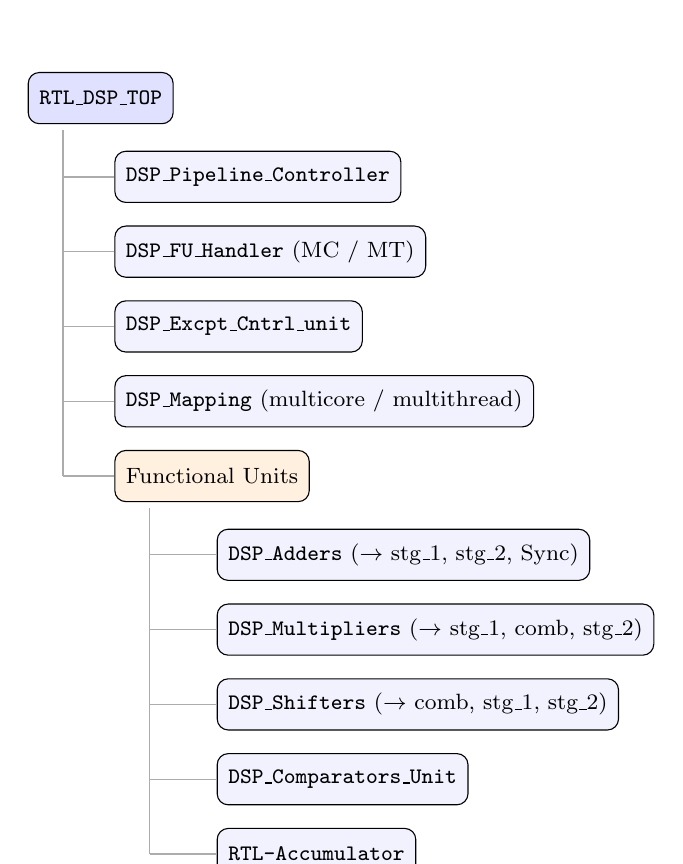
\begin{tikzpicture}[
  comp/.style={draw, rounded corners, fill=blue!5, inner sep=4pt, anchor=west,
               font=\footnotesize, minimum height=6.5mm},
  topb/.style={comp, fill=blue!12},
  fub/.style={comp, fill=orange!12},
  bus/.style={draw, gray!65, line width=0.5pt}
]
% --- level 0 ---
\node[topb] (top) at (0,0) {\texttt{RTL\_DSP\_TOP}};
% --- level 1 (children of TOP) ---
\node[comp] (pc) at (1.1,-1.00) {\texttt{DSP\_Pipeline\_Controller}};
\node[comp] (fh) at (1.1,-1.95) {\texttt{DSP\_FU\_Handler} (MC / MT)};
\node[comp] (ex) at (1.1,-2.90) {\texttt{DSP\_Excpt\_Cntrl\_unit}};
\node[comp] (mp) at (1.1,-3.85) {\texttt{DSP\_Mapping} (multicore / multithread)};
\node[fub]  (fu) at (1.1,-4.80) {Functional Units};
% --- level 2 (children of Functional Units) ---
\node[comp] (add) at (2.4,-5.80) {\texttt{DSP\_Adders} ($\rightarrow$ stg\_1, stg\_2, Sync)};
\node[comp] (mul) at (2.4,-6.75) {\texttt{DSP\_Multipliers} ($\rightarrow$ stg\_1, comb, stg\_2)};
\node[comp] (shf) at (2.4,-7.70) {\texttt{DSP\_Shifters} ($\rightarrow$ comb, stg\_1, stg\_2)};
\node[comp] (cmp) at (2.4,-8.65) {\texttt{DSP\_Comparators\_Unit}};
\node[comp] (acc) at (2.4,-9.60) {\texttt{RTL-Accumulator}};
% --- connectors: level-1 bus drops from TOP, elbows into each child ---
\draw[bus] (0.45,-0.40) -- (0.45,-4.80);
\foreach \y in {-1.00,-1.95,-2.90,-3.85,-4.80}{ \draw[bus] (0.45,\y) -- (1.10,\y); }
% --- connectors: level-2 bus drops from Functional Units ---
\draw[bus] (1.55,-5.20) -- (1.55,-9.60);
\foreach \y in {-5.80,-6.75,-7.70,-8.65,-9.60}{ \draw[bus] (1.55,\y) -- (2.40,\y); }
\end{tikzpicture}
\caption{Re-engineered module hierarchy of the accelerator. Each functional unit
is a self-contained VHDL entity with an explicit interface, exposing a clean
boundary at which redundancy wrappers and sensors can be attached.}
\label{fig:hierarchy}
\end{figure}

\subsection{Why isolation matters}

The decisive property of the re-engineered design is that each functional unit
is an independently instantiable entity with a fully specified port interface.
This has three consequences that the rest of the thesis depends on:

\begin{enumerate}
  \item \textbf{Selective hardening.} A redundancy wrapper can instantiate
        \emph{exactly one} functional unit two or three times and combine the
        copies, without touching any other unit. This is what makes
        per-functional-unit DMR and TMR possible.
  \item \textbf{Composability.} Because the wrappers preserve the original port
        interface, a hardened unit is a drop-in replacement for its unhardened
        counterpart; hardening any subset of units --- or all of them --- is
        simply a matter of choosing which wrappers to instantiate, controlled by
        the top-level \texttt{*\_DMR\_EN} / \texttt{*\_TMR\_EN} constants.
  \item \textbf{Instrumentability.} The same clean boundaries give the IJTAG
        sensor-insertion tool of Chapter~\ref{ch:ijtag} well-defined points at
        which to attach activity and thermal monitors.
\end{enumerate}

The modular hierarchy is thus not merely a tidy refactoring: it is the
enabling substrate for the fault-tolerance framework and the monitoring framework
that follow.

\chapter{Fault-Tolerance Framework: DMR and TMR}
\label{ch:framework}

Building on the modular accelerator of Chapter~\ref{ch:architecture}, this
chapter presents the fault-tolerance framework. Section~\ref{sec:ft-primitives}
introduces the two reusable redundancy primitives. Section~\ref{sec:ft-wrappers}
shows how they wrap the functional units. Section~\ref{sec:ft-scenarioB}
describes per-functional-unit and full-accelerator hardening (Scenario~A), and
Section~\ref{sec:ft-scenarioA} describes replication-based redundancy
(Scenario~B). Section~\ref{sec:ft-control} explains how a configuration is
selected at elaboration time.

\section{Reusable redundancy primitives}
\label{sec:ft-primitives}

The framework rests on two deliberately tiny, technology-independent VHDL
entities. Their smallness is a feature: because each operates on a single bit,
it can be replicated bit-by-bit across an arbitrarily wide datapath, and because
it is purely structural it imposes no constraints on the module it protects.

\subsection{The DMR comparison cell}

The Dual-Modular-Redundancy cell takes the corresponding output bit from two
copies of a module and produces a single result bit together with an error flag.
If the two inputs agree, the result is forwarded and the flag is deasserted; if
they disagree, the flag is asserted to signal a detected error. The complete
entity is shown in Listing~\ref{lst:dmr}.

\begin{lstlisting}[language=myvhdl, caption={The single-bit DMR comparison cell.}, label={lst:dmr}]
entity DMR is
  port(
    in1, in2 : in  std_logic;
    err_flag : out std_logic;
    result   : out std_logic
  );
end entity DMR;

architecture DMR_arch of DMR is
begin
  process(in1, in2)
  begin
    if in1 = in2 then
      result   <= in1;
      err_flag <= '0';  -- no error
    else
      result   <= in1;  -- arbitrary choice
      err_flag <= '1';  -- error detected
    end if;
  end process;
end architecture DMR_arch;
\end{lstlisting}

When the two copies disagree the cell cannot know which is correct, so it
forwards one of them (here \texttt{in1}) and relies on the asserted
\texttt{err\_flag} to trigger a system-level response. The error flags from all
bits of a functional unit are combined so that any single-bit discrepancy raises
the unit-level error indication.

\subsection{The TMR majority voter}

The Triple-Modular-Redundancy cell takes the corresponding output bit from three
copies of a module and outputs the majority value, realising
Equation~\ref{eq:majority}. The complete entity is shown in
Listing~\ref{lst:tmr}.

\begin{lstlisting}[language=myvhdl, caption={The single-bit TMR majority voter.}, label={lst:tmr}]
entity TMR is
  port(
    in1, in2, in3 : in  std_logic;
    result        : out std_logic
  );
end entity TMR;

architecture TMR_arch of TMR is
begin
  result <= (in1 and in2) or (in2 and in3) or (in1 and in3);
end architecture TMR_arch;
\end{lstlisting}

As long as at most one of the three inputs is wrong at any given bit, the
majority output is correct, so the voter \emph{masks} the fault without any need
for a recovery action. Unlike DMR, TMR therefore does not produce an error flag:
correct operation continues transparently.

\section{Wrapping the functional units}
\label{sec:ft-wrappers}

A redundancy \emph{wrapper} is a VHDL entity that exposes exactly the same port
interface as the functional unit it protects, so that it is a drop-in
replacement. Internally, the wrapper instantiates the functional unit two times
(for DMR) or three times (for TMR), drives all copies with identical inputs, and
recombines their outputs bit-by-bit using arrays of the primitive cells of
Section~\ref{sec:ft-primitives}. Figure~\ref{fig:wrappers} illustrates both
arrangements.

\begin{figure}[htbp]
\centering
\begin{subfigure}[t]{0.48\textwidth}
\centering
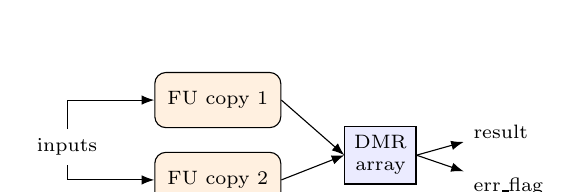
\begin{tikzpicture}[
  box/.style={draw, rounded corners, minimum width=16mm, minimum height=7mm, font=\scriptsize, fill=orange!12, align=center},
  cell/.style={draw, minimum width=9mm, minimum height=7mm, font=\scriptsize, fill=blue!8, align=center},
  arr/.style={-{Latex[length=1.6mm]}}]
\node (in) {\scriptsize inputs};
\node[box, right=6mm of in, yshift=6mm] (a) {FU copy 1};
\node[box, below=3mm of a] (b) {FU copy 2};
\node[cell, right=8mm of a, yshift=-7mm] (d) {DMR\\array};
\node[right=6mm of d, yshift=3mm, font=\scriptsize] (r) {result};
\node[right=6mm of d, yshift=-4mm, font=\scriptsize] (e) {err\_flag};
\draw[arr] (in) |- (a.west);
\draw[arr] (in) |- (b.west);
\draw[arr] (a.east) -- (d.west);
\draw[arr] (b.east) -- (d.west);
\draw[arr] (d.east) -- (r);
\draw[arr] (d.east) -- (e);
\end{tikzpicture}
\caption{DMR wrapper: two copies, bitwise comparison, error flag.}
\end{subfigure}
\hfill
\begin{subfigure}[t]{0.48\textwidth}
\centering
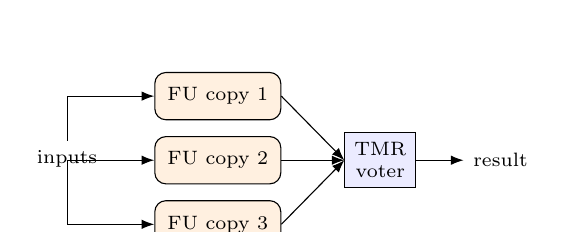
\begin{tikzpicture}[
  box/.style={draw, rounded corners, minimum width=16mm, minimum height=6mm, font=\scriptsize, fill=orange!12, align=center},
  cell/.style={draw, minimum width=9mm, minimum height=7mm, font=\scriptsize, fill=blue!8, align=center},
  arr/.style={-{Latex[length=1.6mm]}}]
\node (in) {\scriptsize inputs};
\node[box, right=6mm of in, yshift=8mm] (a) {FU copy 1};
\node[box, below=2mm of a] (b) {FU copy 2};
\node[box, below=2mm of b] (c) {FU copy 3};
\node[cell, right=8mm of b] (v) {TMR\\voter};
\node[right=6mm of v, font=\scriptsize] (r) {result};
\draw[arr] (in) |- (a.west);
\draw[arr] (in) |- (b.west);
\draw[arr] (in) |- (c.west);
\draw[arr] (a.east) -- (v.west);
\draw[arr] (b.east) -- (v.west);
\draw[arr] (c.east) -- (v.west);
\draw[arr] (v.east) -- (r);
\end{tikzpicture}
\caption{TMR wrapper: three copies, bitwise majority vote.}
\end{subfigure}
\caption{Redundancy wrappers. Each preserves the protected unit's interface, so
hardening is transparent to the rest of the accelerator.}
\label{fig:wrappers}
\end{figure}

Listing~\ref{lst:adder_dmr} sketches the structure of the adder DMR wrapper. The
wrapper declares an internal array type that holds the duplicated outputs, binds
the \texttt{DMR} and \texttt{DSP\_Adders} components, instantiates two adder
copies, and applies the DMR cell across every output bit in a generate loop. The
multiplier, shifter, and comparator wrappers follow exactly the same pattern,
differing only in the width and type of the outputs they recombine.

\begin{lstlisting}[language=myvhdl, caption={Structure of the adder DMR wrapper (abridged).}, label={lst:adder_dmr}]
architecture DSP_Adders_DMR_arch of DSP_Adders_DMR is
  type dmr_type is array (1 downto 0)
       of array_2d_dsp_operands(FU_NUM-1 downto 0);
  signal dmr_dsp_out_adder_results : dmr_type;
  component DMR
    port(in1, in2 : in std_logic; err_flag, result : out std_logic);
  end component;
  component DSP_Adders generic(...); port(...); end component;
begin
  -- two identical copies of the adder functional unit
  ADDER_COPY_0 : DSP_Adders generic map(...) port map(...,
      dsp_out_adder_results => dmr_dsp_out_adder_results(0), ...);
  ADDER_COPY_1 : DSP_Adders generic map(...) port map(...,
      dsp_out_adder_results => dmr_dsp_out_adder_results(1), ...);
  -- bitwise comparison across the whole result vector
  GEN_DMR : for i in ... generate
    DMR_i : DMR port map(
      in1 => dmr_dsp_out_adder_results(0)(...)(i),
      in2 => dmr_dsp_out_adder_results(1)(...)(i),
      result => dsp_out_adder_results(...)(i),
      err_flag => err_flag_vector(i));
  end generate;
end architecture;
\end{lstlisting}

\section{Scenario A: per-functional-unit and full-accelerator hardening}
\label{sec:ft-scenarioB}

In the single-lane accelerator, redundancy is applied by replacing one or more
functional units with their hardened wrappers. The top-level design exposes a
set of Boolean constants --- \texttt{ADDERS\_DMR\_EN}, \texttt{ADDERS\_TMR\_EN},
\texttt{MULTIPLIERS\_DMR\_EN}, \texttt{MULTIPLIERS\_TMR\_EN},
\texttt{SHIFTERS\_DMR\_EN}, \texttt{SHIFTERS\_TMR\_EN},
\texttt{COMPARATORS\_DMR\_EN}, and \texttt{COMPARATORS\_TMR\_EN} --- each of which
selects whether the corresponding unit is instantiated as plain, DMR-wrapped, or
TMR-wrapped. This yields the following configurations, all studied
experimentally:

\begin{itemize}
  \item \textbf{Baseline} --- no constant set; the accelerator is unhardened and
        provides the reference area, power, and timing.
  \item \textbf{Single-FU DMR / TMR} --- exactly one of the four arithmetic
        units (adder, multiplier, shifter, or comparator) is wrapped, the others
        left plain. This isolates the cost of protecting each unit individually.
  \item \textbf{Full DMR / TMR} --- all four arithmetic units are wrapped
        simultaneously, giving the cost of protecting the entire arithmetic
        datapath.
\end{itemize}

Because the four functional units differ greatly in size, single-FU hardening
spans a wide range of costs: protecting the comparator is nearly free, whereas
protecting the multiplier is the dominant contributor to any scheme that
includes it. These differences are quantified in Chapter~\ref{ch:results} and
form the basis of the design guidelines.

\section{Scenario B: replication-based redundancy}
\label{sec:ft-scenarioA}

The second way of obtaining redundancy exploits the accelerator's existing
\emph{performance} replication. With \texttt{replicate\_accl\_en} enabled, three
complete accelerator lanes operate in parallel. Rather than building fresh
copies of each functional unit, the redundancy logic is placed in the
\texttt{DSP\_Mapping} layer, where the results produced by the lanes are already
gathered:

\begin{itemize}
  \item \textbf{Replicated baseline} --- three lanes, results simply mapped out,
        no redundancy logic. This is the throughput-oriented configuration.
  \item \textbf{Replicated + DMR voting} --- the mapping layer compares lane
        outputs and raises an error flag on disagreement.
  \item \textbf{Replicated + TMR voting} --- the mapping layer majority-votes the
        three lane outputs, masking any single faulty lane.
\end{itemize}

The mapping unit toggles between these through its own \texttt{DMR\_ENABLED} and
\texttt{TMR\_ENABLED} constants. The crucial observation --- borne out by the
results --- is that since the costly datapath copies already exist for
throughput, the \emph{incremental} cost of adding voting is only the cost of the
comparators or voters in the mapping layer, which is small relative to the
replicated datapath.

\section{Selecting a configuration at elaboration}
\label{sec:ft-control}

A complete experimental configuration is therefore defined by two groups of
settings: the top-level \texttt{replicate\_accl\_en} generic (Scenario~B versus
Scenario~A) and, within each scenario, the redundancy-enable constants. Because
all of these are resolved at \emph{elaboration} time, switching configurations
requires no change to the functional logic --- only a change of constants --- and
each configuration elaborates into a distinct, fully synthesisable netlist. The
synthesis sweep of Chapter~\ref{ch:experiment} automates exactly this: it edits
the relevant constants, elaborates, and synthesises, sweeping the full
configuration matrix across all technology nodes. The complete matrix is listed
in Table~\ref{tab:matrix}.

\begin{table}[htbp]
\centering
\caption{Complete configuration matrix explored in this work. Each configuration is synthesised at all three technology nodes, for a total of 42 synthesis runs.}
\label{tab:matrix}
\small
\begin{tabular}{llp{7.5cm}}
\toprule
Scenario & Configuration & Description \\
\midrule
A (single core) & Baseline & Unhardened reference accelerator \\
 & Adder DMR / TMR & Redundancy on the adder functional unit only \\
 & Multiplier DMR / TMR & Redundancy on the multiplier functional unit only \\
 & Shifter DMR / TMR & Redundancy on the shifter functional unit only \\
 & Comparator DMR / TMR & Redundancy on the comparator functional unit only \\
 & Full DMR / TMR & Redundancy applied to all functional units simultaneously \\
B (replicated) & Replicated baseline & Three accelerator lanes, no voting \\
 & Replicated + DMR & Three lanes with duplication-comparison in the mapping unit \\
 & Replicated + TMR & Three lanes with majority voting in the mapping unit \\
\bottomrule
\end{tabular}
\end{table}


\chapter{In-Field Monitoring with Automated IJTAG Instrumentation}
\label{ch:ijtag}

Structural redundancy keeps the accelerator \emph{correct} in the presence of
faults; it does not, on its own, make the accelerator \emph{observable}. For
in-field health management --- tracking temperature, activity, and degradation
over the service life, and reacting before a marginal condition becomes a failure
--- the design must expose internal state through a standard, retargetable
access mechanism. This chapter presents the second framework of the thesis: an
automated flow that inserts IEEE~1687 (IJTAG) sensors into the accelerator's
VHDL hierarchy and builds the on-chip access network around them.

Section~\ref{sec:ij-goal} states the goal and the manual-effort problem it
solves. Section~\ref{sec:ij-sensor} describes the sensor instrument.
Section~\ref{sec:ij-tool} describes the insertion tool and its
configuration. Section~\ref{sec:ij-flow} describes the two-phase Tessent flow
that builds the network. Section~\ref{sec:ij-synth} reports the synthesis cost of
the instrumentation.

\section{Goal: observability without manual rewiring}
\label{sec:ij-goal}

Attaching even a single instrument to an IJTAG network by hand is tedious and
error-prone: the instrument must be declared, instantiated at the right point in
the hierarchy, connected to the scan path with the correct client-interface
signals, described in ICL so that the tool can retarget access to it, and hosted
behind a Segment Insertion Bit (SIB) so it can be switched in and out of the
active chain. Doing this for several instruments scattered across a deep
hierarchy --- and redoing it every time the design changes --- quickly becomes
unmanageable.

The flow developed here removes the manual effort entirely. The designer marks
\emph{where} sensors should go using lightweight pragmas in the VHDL and
\emph{describes} the sensors and their connections once in a JSON configuration
file. A Python tool then performs the mechanical work --- filling in
declarations and instantiations, producing modified source files --- and emits
the Tessent scripts that extract the connectivity and synthesise the IJTAG
network automatically.

\section{The sensor instrument}
\label{sec:ij-sensor}

The instrument used in this work is an \emph{activity sensor}: a small monitor
that counts rising-edge toggle events on a chosen internal signal over a window
and exposes the count, together with an \texttt{alert} bit, through a proper
IJTAG Test Data Register (TDR). Conceptually the same wrapper accommodates other
sensor types --- a thermal monitor, for instance --- since all that the network
sees is a standard 1687 client interface.

The instrument has two clearly separated parts, illustrated in
Figure~\ref{fig:sensor}:

\begin{itemize}
  \item A \textbf{functional side}, clocked by the design clock, which observes
        the monitored signal and maintains the activity counter and alert.
  \item An \textbf{IJTAG client side}, clocked by the scan clock \texttt{tck},
        comprising the TDR and the standard 1687 control signals
        (\texttt{reset}, \texttt{sel}, \texttt{ce}, \texttt{se}, \texttt{si},
        \texttt{so}). At capture time the TDR samples \{\texttt{alert},
        \texttt{activity\_count}\}; the value is then shifted out through the
        network.
\end{itemize}

\begin{figure}[htbp]
\centering
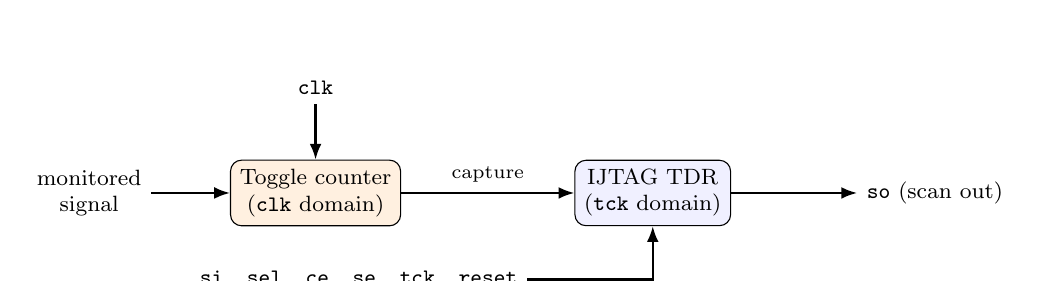
\begin{tikzpicture}[
  box/.style={draw, rounded corners, minimum height=8mm, align=center, font=\footnotesize, fill=blue!6},
  arr/.style={-{Latex[length=2mm]}, thick}]
\node[box, fill=orange!12] (cnt) {Toggle counter\\(\texttt{clk} domain)};
\node[box, right=22mm of cnt] (tdr) {IJTAG TDR\\(\texttt{tck} domain)};
\node[left=10mm of cnt, font=\footnotesize, align=center] (sig) {monitored\\signal};
\node[above=7mm of cnt, font=\footnotesize] (clk) {\texttt{clk}};
\node[right=16mm of tdr, font=\footnotesize] (so) {\texttt{so} (scan out)};
\node[left=6mm of tdr, yshift=-11mm, font=\footnotesize] (si) {\texttt{si, sel, ce, se, tck, reset}};
\draw[arr] (sig) -- (cnt);
\draw[arr] (clk) -- (cnt);
\draw[arr] (cnt) -- node[above, font=\scriptsize] {capture} (tdr);
\draw[arr] (tdr) -- (so);
\draw[arr] (si) -| (tdr.south);
\end{tikzpicture}
\caption{Activity-sensor instrument. The functional counter is sampled into an
IEEE~1687 Test Data Register, which is accessed serially through the standard
client interface driven by the IJTAG network.}
\label{fig:sensor}
\end{figure}

A deliberate design choice is that every IJTAG \emph{input} of the instrument
carries a default value in its port declaration. This allows the instance to be
left with open associations in plain RTL --- the functional simulation and the
Design Compiler elaboration both accept it --- while Tessent connects the client
interface when it inserts the scan network. The instrument is thus valid both
before and after network insertion, which is what makes a clean,
synthesise-anywhere flow possible.

\section{The sensor-insertion tool}
\label{sec:ij-tool}

\subsection{Pragma-marked injection points}

The designer indicates where a sensor's declaration and instantiation should
appear by placing pragma comments in the relevant VHDL files. The tool scans the
hierarchy for these pragmas and replaces them with the concrete declaration and
instantiation generated from the configuration. Because the markers are
comments, an un-instrumented build is completely unaffected.

\subsection{JSON configuration}

A single \texttt{config.json} file describes everything the tool needs: the
top-level entity and working directory, the clock port and period, the cell
libraries and packages, the list of sensor types and their ICL port names, and
--- crucially --- the set of \emph{instances} to create. Each instance names the
sensor type, the generic map (sensor identifier and counter-window width), the
port map binding the instrument's functional ports to real design signals, and
the hierarchical \texttt{tessent\_path} at which the instrument lives.

In this study three activity-sensor instances are defined at three different
levels of the hierarchy, demonstrating that the flow works at arbitrary depth:

\begin{enumerate}
  \item \texttt{act\_sensor\_top} --- at the top level
        (\texttt{/RTL\_DSP\_TOP}), monitoring the accelerator busy signal.
  \item \texttt{act\_sensor\_adders} --- one level down, inside
        \texttt{DSP\_Adders}, monitoring the adder enable.
  \item \texttt{act\_sensor\_adders\_sync} --- two levels down, inside the
        adder synchronisation block, monitoring the adder enable vector.
\end{enumerate}

A \texttt{configurations} section then groups these instances into cumulative
build variants --- \texttt{1sensor}, \texttt{2sensor}, and \texttt{3sensor} ---
so that the cost of progressively adding instruments can be measured (see
Section~\ref{sec:ij-synth}). The relationship is summarised in
Table~\ref{tab:sensors}.

\begin{table}[htbp]
\centering
\caption{Sensor instances and the cumulative build configurations. Each
configuration adds one more activity sensor, at a progressively deeper point in
the hierarchy.}
\label{tab:sensors}
\small
\begin{tabular}{llp{6.0cm}}
\toprule
Build & Instances & Deepest instrumentation point \\
\midrule
\texttt{1sensor} & top                          & \texttt{/RTL\_DSP\_TOP} \\
\texttt{2sensor} & top, adders                  & \texttt{/RTL\_DSP\_TOP/DSP\_Adders} \\
\texttt{3sensor} & top, adders, adders\_sync    & \texttt{.../DSP\_Adders\_Sync\_inst} \\
\bottomrule
\end{tabular}
\end{table}

\subsection{What the tool emits}

For a chosen configuration, the tool writes a set of \emph{modified} VHDL files
(originals untouched) with the pragmas filled in, and generates the Tessent
dofiles for the next phase: an ICL-extraction script per sensor and a single
\texttt{inject\_sensors.tcl} insertion script. A companion driver script then
runs the whole flow --- ICL extraction, IJTAG insertion, and Design Compiler
synthesis --- for every configuration found beside it, capturing and scanning
each step's log for errors.

\section{Building the network: the two-phase Tessent flow}
\label{sec:ij-flow}

Constructing the IJTAG network is done in two phases, reflecting how Tessent
consumes instrument descriptions.

\paragraph{Phase 1 --- ICL extraction.} Each sensor's RTL is read and its
Instrument Connectivity Language (ICL) description is extracted, so that the
tool knows the instrument's scan interface and register layout. This produces a
per-sensor ICL module that the insertion phase can reference.

\paragraph{Phase 2 --- IJTAG insertion.} The full design is read in DFT context;
the previously extracted ICL is read back; and Tessent hosts each instrument
behind a Segment Insertion Bit, wiring the client interfaces into a hierarchical
scan path and connecting it to the top-level TAP. The result is a design in which
all sensors are reachable through one standard IJTAG port, and the access network
can be reconfigured (via the SIBs) to include only the instruments of interest.

The flow encodes several hard-won practical details: the cell libraries are read
as Tessent \texttt{tcelllib} files; VHDL-2008 parsing is enabled; the scan clock
is left for the network to drive rather than being constrained as a functional
clock; and the open-by-default IJTAG inputs of the instrument (Section
\ref{sec:ij-sensor}) let the same instrument elaborate cleanly in all tools.
Figure~\ref{fig:ijtag-flow} summarises the end-to-end flow.

\begin{figure}[htbp]
\centering
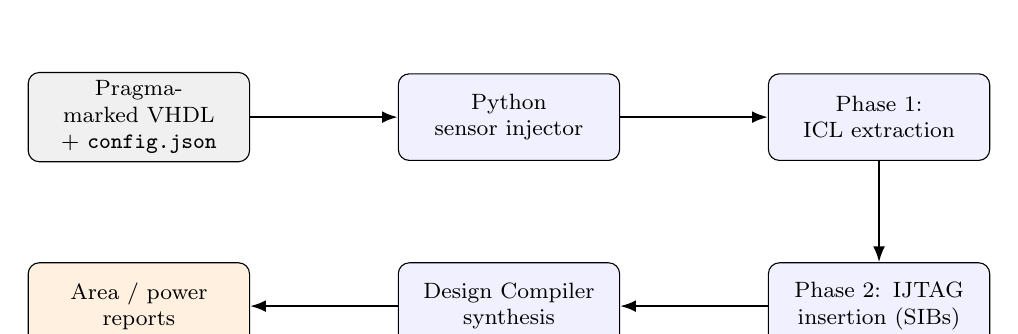
\begin{tikzpicture}[
  flowbox/.style={draw, rounded corners, text width=2.6cm, align=center,
                  minimum height=11mm, inner sep=3pt, font=\footnotesize, fill=blue!6},
  arr/.style={-{Latex[length=2mm]}, thick}]
\node[flowbox, fill=gray!12] (vhdl) at (0,0)    {Pragma-marked VHDL\\+ \texttt{config.json}};
\node[flowbox]               (inj)  at (4.7,0)   {Python\\sensor injector};
\node[flowbox]               (icl)  at (9.4,0)   {Phase 1:\\ICL extraction};
\node[flowbox]               (ins)  at (9.4,-2.4) {Phase 2: IJTAG\\insertion (SIBs)};
\node[flowbox]               (dc)   at (4.7,-2.4) {Design Compiler\\synthesis};
\node[flowbox, fill=orange!12] (rep) at (0,-2.4)  {Area / power\\reports};
\draw[arr] (vhdl) -- (inj);
\draw[arr] (inj) -- (icl);
\draw[arr] (icl) -- (ins);
\draw[arr] (ins) -- (dc);
\draw[arr] (dc) -- (rep);
\end{tikzpicture}
\caption{End-to-end automated IJTAG instrumentation flow, from pragma-marked
VHDL to synthesis reports. The injector also emits the synthesis scripts that
drive the final Design Compiler step.}
\label{fig:ijtag-flow}
\end{figure}

\section{Synthesis cost of the instrumentation}
\label{sec:ij-synth}

To quantify the hardware cost of observability, each instrumented configuration
(\texttt{1sensor}, \texttt{2sensor}, \texttt{3sensor}) was synthesised at all
three technology nodes in two accounting modes: \emph{black box}, in which the
sensor instruments are treated as empty boxes, and \emph{counted}, in which they
are synthesised and their cells counted. The difference between the two is the
synthesised cost of the sensor logic plus the IJTAG access-network glue. The
results are collected in Table~\ref{tab:ijtag} and plotted in
Figure~\ref{fig:ijtag-cost}.

\begin{table}[htbp]
\centering
\caption{Area cost of the IEEE~1687 sensor instrumentation. \emph{Counted} synthesises the sensor instruments fully; \emph{black box} treats them as empty. Their difference is the synthesised cost of the sensors plus the IJTAG access network. The cost is about 1.7\% at the mature node and falls within synthesis optimisation noise at the finer nodes.}
\label{tab:ijtag}
\small
\begin{tabular}{llrrr}
\toprule
Node & Sensors & Counted area & Black-box area & Instrument cost (\%) \\
\midrule
IHP 130\,nm & 1 & 1,029,222 & 1,012,067 & +1.70 \\
 & 2 & 1,029,242 & 1,012,127 & +1.69 \\
 & 3 & 1,023,080 & 1,012,067 & +1.09 \\
\midrule
NanGate 45\,nm & 1 & 83,981 & 84,401 & -0.50 \\
 & 2 & 84,127 & 84,569 & -0.52 \\
 & 3 & 84,127 & 85,071 & -1.11 \\
\midrule
NanGate 15\,nm & 1 & 21,764 & 21,809 & -0.21 \\
 & 2 & 21,764 & 21,852 & -0.40 \\
 & 3 & 21,764 & 21,979 & -0.98 \\
\bottomrule
\end{tabular}
\end{table}


\begin{figure}[htbp]
\centering
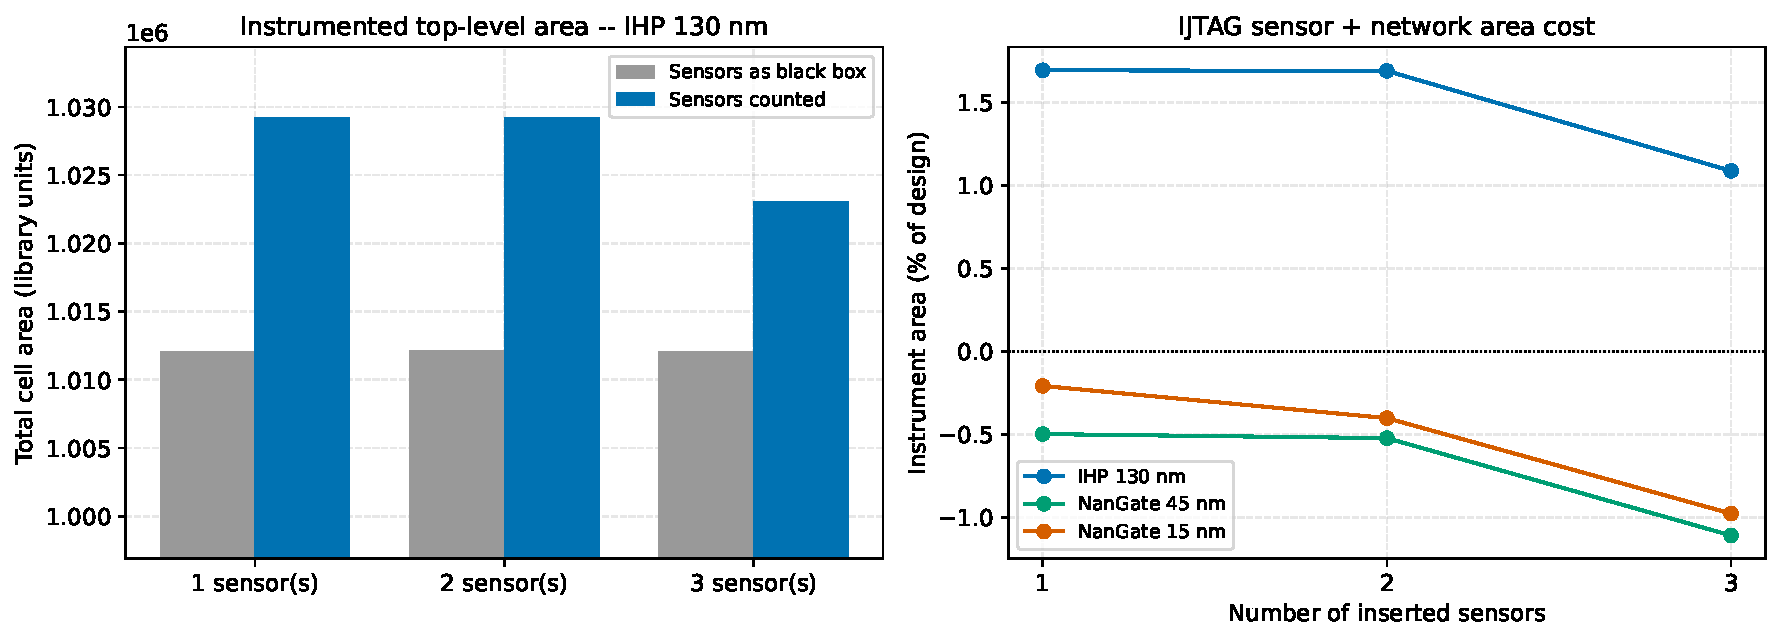
\includegraphics[width=\textwidth]{img/plots/ijtag_cost.pdf}
\caption{Area cost of the IJTAG sensor instrumentation. Left: counted versus
black-box top-level area at the mature node, where the sensor logic is visible
as a small increment. Right: the instrument cost as a percentage of the design,
versus the number of inserted sensors, for the three nodes.}
\label{fig:ijtag-cost}
\end{figure}

Two observations follow. First, the absolute cost of the instrumentation is
\emph{small}: at the mature node the sensors plus network amount to roughly
$1.7\%$ of the (replicated) design, and adding further sensors changes this only
marginally, because the per-sensor logic --- an eight-bit counter and a short TDR
--- is tiny next to a multi-lane vector accelerator. Second, at the finer nodes
the measured difference between the counted and black-box builds falls
\emph{within the run-to-run noise} of synthesis optimisation (it is sub-percent
and can even appear slightly negative, when the optimiser happens to share or
restructure logic differently between the two builds). The honest conclusion is
that, on a design of this size, the area cost of IJTAG-based observability is
negligible-to-minor. In-field monitoring can therefore be added essentially
``for free'' relative to the redundancy overheads quantified in
Chapter~\ref{ch:results}, which makes combining the two frameworks on the same
accelerator very attractive.

\chapter{Experimental Setup}
\label{ch:experiment}

This chapter describes how the configurations of Chapters~\ref{ch:framework} and
\ref{ch:ijtag} are turned into quantitative data. Section~\ref{sec:ex-flow}
describes the synthesis flow and tools. Section~\ref{sec:ex-nodes} describes the
three technology nodes. Section~\ref{sec:ex-matrix} defines the configuration
matrix. Section~\ref{sec:ex-metrics} defines the metrics and the normalisation
used throughout the results. Section~\ref{sec:ex-auto} describes the automation
that makes the sweep reproducible.

\section{Synthesis flow and tools}
\label{sec:ex-flow}

All configurations are functionally elaborated from the same VHDL-2008 source
base and synthesised with Synopsys Design Compiler~\cite{designcompiler}. For each configuration the
flow reads the technology library and the design packages, analyses and
elaborates the top-level accelerator with the chosen generics and redundancy
constants, compiles to the target standard-cell library, and writes a fixed set
of reports --- area, cell counts, references, resources, power, and timing.

Each configuration is synthesised against the same fixed, deliberately
aggressive clock constraint at a given node, so that the synthesis effort is
identical across all configurations. Because the target period is intentionally
tighter than the design can meet, every configuration reports a (negative) slack;
slack is therefore \emph{not} a useful discriminator here. Instead, the timing
figure of merit used throughout is the \emph{critical-path (data-arrival) delay}
of the longest path, which the tool reports regardless of slack. Since the same
constraint and effort are applied to every configuration at a node, the
data-arrival delays are directly comparable, and their ratio to the baseline
captures exactly how much each redundancy scheme lengthens the critical path. The
voters and comparators of DMR/TMR are thin combinational layers on the
functional-unit outputs, so they are expected to add little to the critical path
--- a hypothesis the results confirm.

\section{Technology nodes}
\label{sec:ex-nodes}

To test whether the cost of redundancy is stable across process generations, each
configuration is synthesised at three nodes spanning a wide range of maturity:

\begin{itemize}
  \item \textbf{IHP 130\,nm} (\texttt{sg13g2})~\cite{ihp} --- a mature, open
        process-design-kit node, representative of robust, cost-sensitive and
        radiation-tolerant designs.
  \item \textbf{NanGate 45\,nm}~\cite{nangate} --- an open, widely used academic
        standard-cell library representative of a mainstream node.
  \item \textbf{NanGate 15\,nm}~\cite{nangate} --- an open FinFET-era library representative of
        an advanced node.
\end{itemize}

These three points let the study distinguish effects that are intrinsic to the
\emph{architecture} of the redundancy schemes (and therefore stable across nodes)
from effects that depend on the \emph{technology}. A practical consequence of
mixing such different libraries is that their reporting units differ --- dynamic
power is reported in milliwatts at two nodes and microwatts at another, and the
advanced library reports timing and power on a different absolute scale. The
analysis handles this by reading the units from each report and, wherever
absolute values are compared across nodes, by \emph{normalising to the per-node
baseline} so that unit and scale differences cancel.

\section{Configuration matrix}
\label{sec:ex-matrix}

The full sweep is the Cartesian product of the configurations and the technology
nodes. The configurations comprise the two scenarios introduced in
Chapter~\ref{ch:framework}:

\begin{itemize}
  \item \textbf{Scenario~A (single core)} --- baseline; each of the four
        arithmetic units (adder, multiplier, shifter, comparator) hardened
        individually with DMR and with TMR; and the full datapath hardened with
        DMR and with TMR. This is eleven configurations.
  \item \textbf{Scenario~B (replicated)} --- replicated baseline; replicated with
        DMR voting; replicated with TMR voting. This is three configurations.
\end{itemize}

Fourteen configurations at three nodes give \textbf{42 synthesis runs} for the
redundancy study, complemented by the \textbf{18 instrumented runs} of
Chapter~\ref{ch:ijtag} (three sensor counts $\times$ three nodes $\times$ two
accounting modes). The redundancy matrix was already listed in
Table~\ref{tab:matrix}.

\section{Metrics and normalisation}
\label{sec:ex-metrics}

From each run the following metrics are extracted:

\begin{itemize}
  \item \textbf{Area.} Total cell area, decomposed into combinational,
        buffer/inverter, sequential (non-combinational), and net-interconnect
        area; plus the number of total, combinational, and sequential cells.
  \item \textbf{Power.} Switching, internal, and leakage power, and their total,
        all normalised to milliwatts by reading each report's unit declarations.
        Power is reported by Design Compiler's hierarchical power analysis with
        default switching activity, so the absolute values are estimates; the
        \emph{ratios} between configurations are the meaningful quantity.
  \item \textbf{Timing.} The critical-path (data-arrival) delay of the longest
        path, used in preference to slack as discussed in
        Section~\ref{sec:ex-flow}.
\end{itemize}

Throughout the results, the headline figure of merit is the \emph{overhead
factor} --- the metric of a hardened configuration divided by the metric of the
baseline \emph{at the same node}. Normalising in this way removes both the
absolute-scale differences between libraries and any common-mode contribution of
the surrounding core, isolating the cost attributable to redundancy itself.

\section{Automation and reproducibility}
\label{sec:ex-auto}

Running 42 synthesis jobs by hand, each requiring a precise combination of
generics and redundancy constants, would be both tedious and unreliable. The
sweep is therefore fully automated by a driver that, for each (node,
configuration) pair, edits the relevant source constants, invokes Design
Compiler, and files the resulting reports into a clearly named directory. The
two scenarios are handled by the same driver: for Scenario~B it toggles the
mapping-layer \texttt{DMR\_ENABLED}/\texttt{TMR\_ENABLED} constants with
replication enabled, and for Scenario~A it toggles the per-unit
\texttt{*\_DMR\_EN}/\texttt{*\_TMR\_EN} constants with replication disabled. The
source files it edits are backed up before any change and restored when the
sweep finishes --- even on error or interruption --- so the working tree is
always left clean. The data-reduction and plotting scripts described in
Appendix~\ref{app:tools} then parse every report into a single table and
generate the figures and tables of the next chapter directly from it, so that
the entire path from raw reports to thesis figures is reproducible by re-running
two scripts.

\chapter{Results and Discussion}
\label{ch:results}

This chapter presents and interprets the design-space exploration. It is
organised from the fine grain outward: Section~\ref{sec:res-fu} examines the cost
of hardening individual functional units; Section~\ref{sec:res-full} the cost of
hardening the full datapath; Section~\ref{sec:res-comp} the composition of that
cost in terms of cells, area, and power; Section~\ref{sec:res-timing} the timing
impact; Section~\ref{sec:res-tradeoff} the area--power trade-off;
Section~\ref{sec:res-repl} the replication scenario; and
Section~\ref{sec:res-nodes} the stability of the findings across nodes.
Section~\ref{sec:res-guidelines} distils the results into design guidelines.
Unless stated otherwise, every quantity is the overhead factor relative to the
per-node baseline, as defined in Section~\ref{sec:ex-metrics}.

\section{Per-functional-unit hardening}
\label{sec:res-fu}

Figure~\ref{fig:fu-area} shows the cell-area overhead of hardening each
functional unit individually, for DMR and TMR, at the three nodes;
Figure~\ref{fig:fu-power} shows the corresponding total-power overhead. The
single most important result of the whole study is visible immediately: \emph{the
cost of redundancy is dominated by which unit is hardened, not merely by whether
DMR or TMR is chosen.}

\begin{figure}[htbp]
\centering
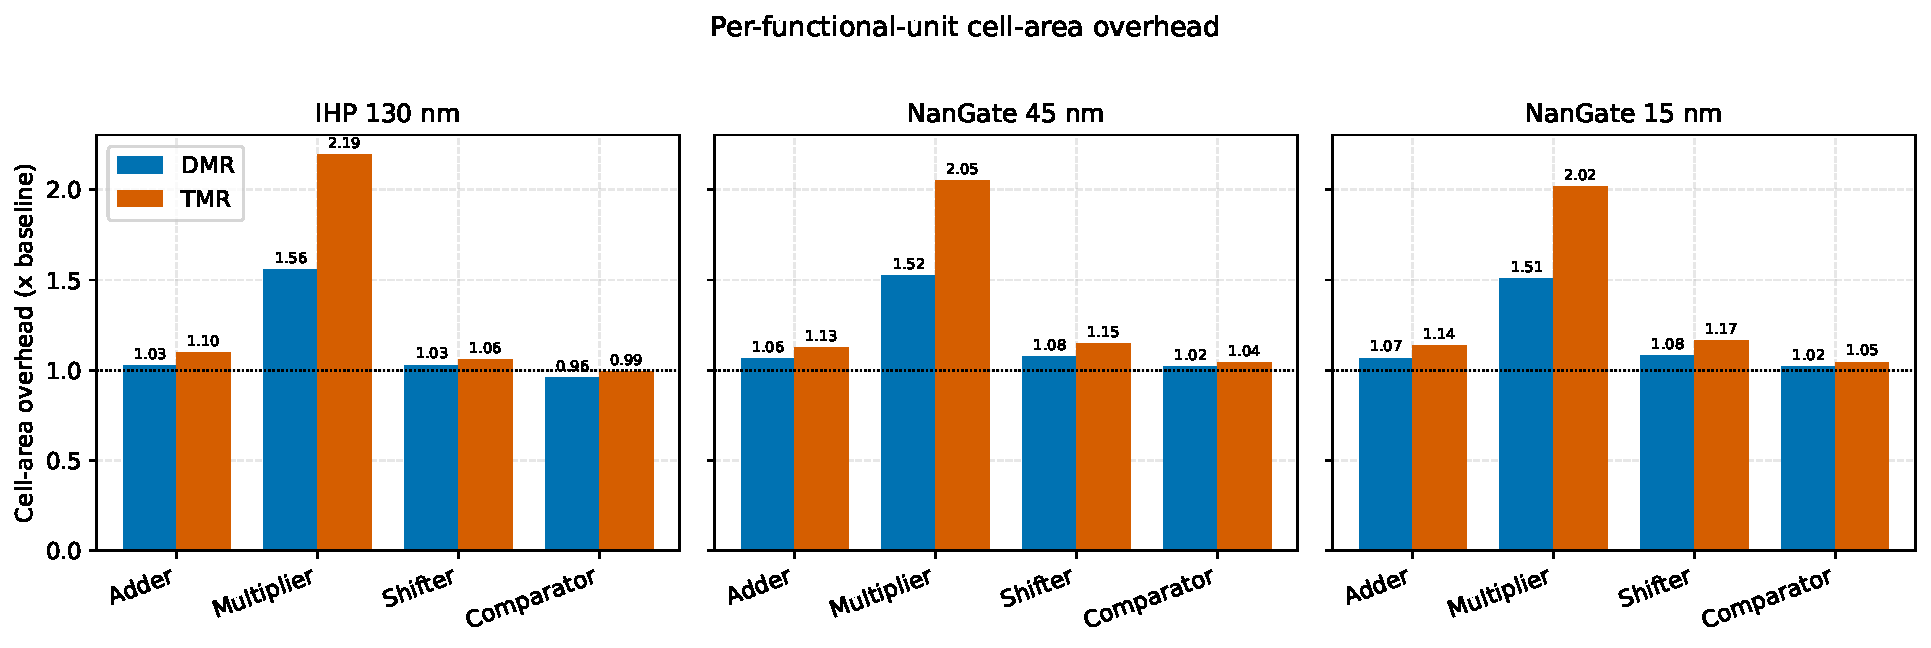
\includegraphics[width=\textwidth]{img/plots/fu_area_overhead.pdf}
\caption{Cell-area overhead of hardening each functional unit individually,
relative to the per-node baseline. The multiplier dominates; the comparator is
almost free. The pattern is essentially identical across the three nodes.}
\label{fig:fu-area}
\end{figure}

\begin{figure}[htbp]
\centering
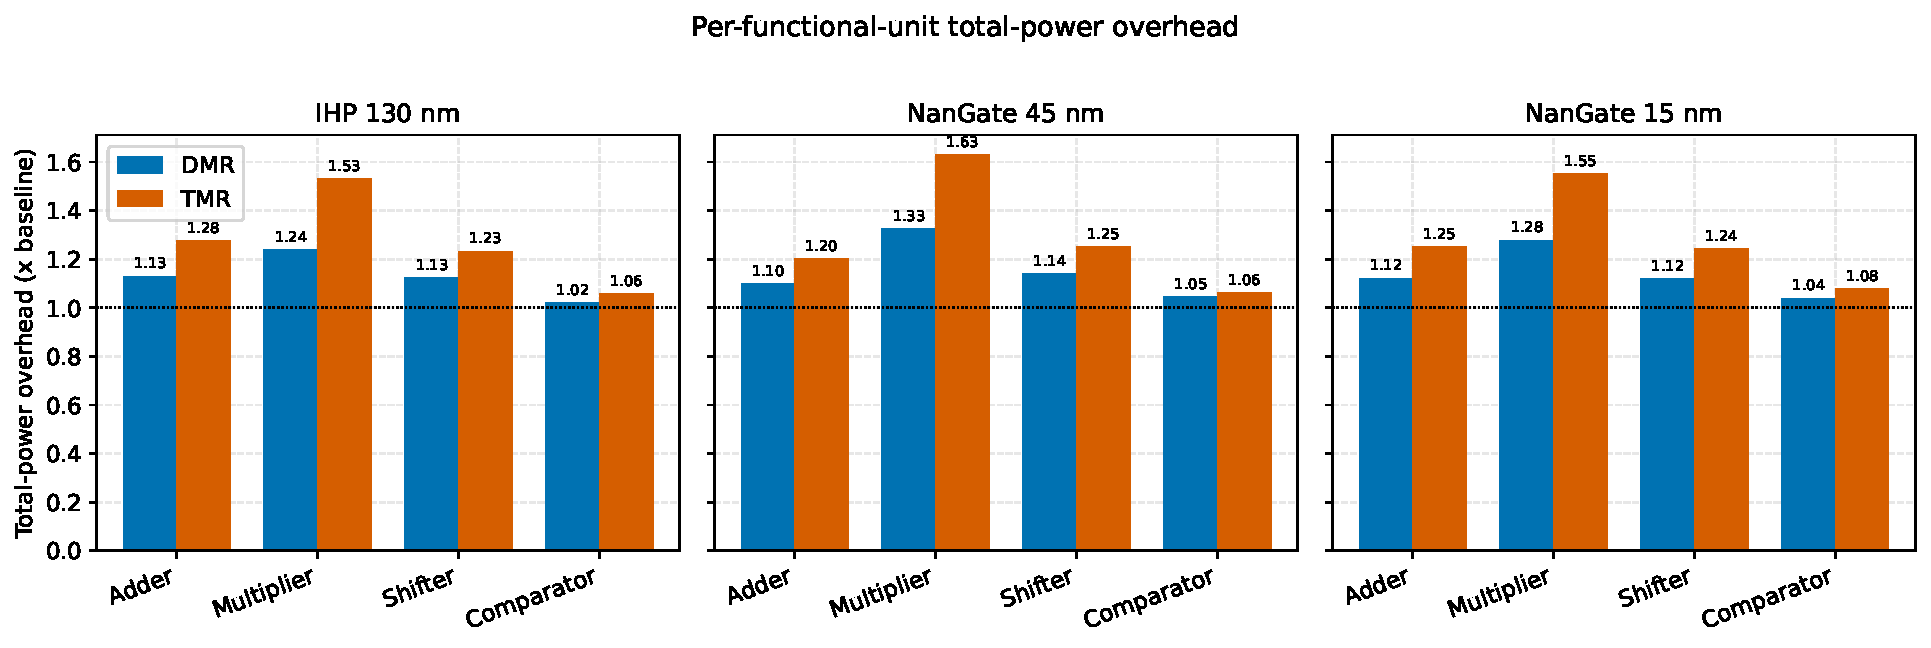
\includegraphics[width=\textwidth]{img/plots/fu_power_overhead.pdf}
\caption{Total-power overhead of hardening each functional unit individually,
relative to the per-node baseline.}
\label{fig:fu-power}
\end{figure}

The \textbf{multiplier} is by far the most expensive unit to protect. At the
mature node, multiplier DMR raises the total cell area to roughly $1.56\times$
the baseline and multiplier TMR to roughly $2.19\times$ --- meaning the
multiplier alone accounts for about half of the entire accelerator's area, so
duplicating it adds about half a baseline and triplicating it adds about a full
baseline. The \textbf{adder} and \textbf{shifter} are moderate and very similar
to each other (DMR around $1.03$--$1.08\times$, TMR around $1.06$--$1.17\times$),
reflecting their comparable, modest size. The \textbf{comparator} is the
cheapest: its DMR and TMR change the total area by only a few percent, and at the
mature node the comparator-DMR area even falls marginally \emph{below} the
baseline ($0.96\times$) --- the logic added is so small that it is lost in the
run-to-run variation of synthesis optimisation. The comparator is the smallest
arithmetic unit and reuses information already produced by the adder, so
protecting it is essentially free.

The same ordering holds for power (Figure~\ref{fig:fu-power}), and the power
overheads remain \emph{smaller} than the area overheads --- multiplier TMR, for
example, costs about $2.19\times$ the area but only about $1.53\times$ the power
at the mature node. The reason is that the duplicated copies are not all
maximally active simultaneously, and a large part of the accelerator's power
(control, mapping, scratchpad interface) is unaffected by datapath redundancy,
so the relative power increase is diluted. Tables~\ref{tab:abs_130nm},
\ref{tab:abs_45nm}, and \ref{tab:abs_15nm} give the underlying absolute numbers
for the three nodes.

\begin{table}[htbp]
\centering
\caption{Synthesis results for the single-core fault-tolerance configurations at IHP 130\,nm. Area is in library units, power in mW, and delay is the critical-path (data-arrival) time in the library time unit.}
\label{tab:abs_130nm}
\small
\begin{tabular}{lrrrrr}
\toprule
Configuration & Cell area & Comb. cells & Seq. cells & Power (mW) & Delay \\
\midrule
Baseline & 361,737 & 32,295 & 1,328 & 20.41 & 4.91 \\
Adder DMR & 371,068 & 32,264 & 1,568 & 23.05 & 5.04 \\
Adder TMR & 396,685 & 33,658 & 1,808 & 26.04 & 4.99 \\
Multiplier DMR & 562,749 & 52,269 & 1,648 & 25.27 & 5.11 \\
Multiplier TMR & 793,544 & 75,388 & 1,968 & 31.24 & 5.14 \\
Shifter DMR & 372,255 & 32,459 & 1,520 & 22.97 & 5.02 \\
Shifter TMR & 382,853 & 32,697 & 1,712 & 25.17 & 5.15 \\
Comparator DMR & 347,479 & 30,652 & 1,392 & 20.83 & 5.08 \\
Comparator TMR & 359,507 & 31,555 & 1,456 & 21.61 & 4.99 \\
Full DMR & 591,559 & 52,962 & 2,144 & 31.36 & 5.21 \\
Full TMR & 871,559 & 78,796 & 2,960 & 42.80 & 5.20 \\
\bottomrule
\end{tabular}
\end{table}

\begin{table}[htbp]
\centering
\caption{Synthesis results for the single-core fault-tolerance configurations at NanGate 45\,nm. Area is in library units, power in mW, and delay is the critical-path (data-arrival) time in the library time unit.}
\label{tab:abs_45nm}
\small
\begin{tabular}{lrrrrr}
\toprule
Configuration & Cell area & Comb. cells & Seq. cells & Power (mW) & Delay \\
\midrule
Baseline & 28,112 & 16,497 & 1,328 & 5.16 & 2.97 \\
Adder DMR & 29,895 & 17,077 & 1,568 & 5.67 & 2.97 \\
Adder TMR & 31,667 & 17,701 & 1,808 & 6.20 & 2.99 \\
Multiplier DMR & 42,867 & 24,816 & 1,648 & 6.84 & 3.02 \\
Multiplier TMR & 57,640 & 33,311 & 1,968 & 8.41 & 3.03 \\
Shifter DMR & 30,262 & 17,698 & 1,520 & 5.88 & 2.94 \\
Shifter TMR & 32,230 & 18,755 & 1,712 & 6.46 & 2.99 \\
Comparator DMR & 28,716 & 16,835 & 1,392 & 5.40 & 2.97 \\
Comparator TMR & 29,303 & 17,188 & 1,456 & 5.48 & 2.99 \\
Full DMR & 47,283 & 26,677 & 2,144 & 8.11 & 2.97 \\
Full TMR & 66,351 & 37,111 & 2,960 & 11.20 & 3.02 \\
\bottomrule
\end{tabular}
\end{table}

\begin{table}[htbp]
\centering
\caption{Synthesis results for the single-core fault-tolerance configurations at NanGate 15\,nm. Area is in library units, power in mW, and delay is the critical-path (data-arrival) time in the library time unit.}
\label{tab:abs_15nm}
\small
\begin{tabular}{lrrrrr}
\toprule
Configuration & Cell area & Comb. cells & Seq. cells & Power (mW) & Delay \\
\midrule
Baseline & 7,254 & 14,199 & 1,328 & 1.69 & 456.39 \\
Adder DMR & 7,746 & 14,812 & 1,568 & 1.90 & 456.39 \\
Adder TMR & 8,238 & 15,458 & 1,808 & 2.11 & 456.40 \\
Multiplier DMR & 10,936 & 20,737 & 1,648 & 2.16 & 460.63 \\
Multiplier TMR & 14,620 & 27,410 & 1,968 & 2.62 & 461.10 \\
Shifter DMR & 7,848 & 15,542 & 1,520 & 1.89 & 454.14 \\
Shifter TMR & 8,452 & 17,060 & 1,712 & 2.10 & 454.14 \\
Comparator DMR & 7,418 & 14,483 & 1,392 & 1.76 & 457.53 \\
Comparator TMR & 7,585 & 14,902 & 1,456 & 1.82 & 455.71 \\
Full DMR & 12,188 & 22,986 & 2,144 & 2.65 & 458.43 \\
Full TMR & 17,136 & 32,251 & 2,960 & 3.59 & 458.38 \\
\bottomrule
\end{tabular}
\end{table}


\section{Full-accelerator hardening}
\label{sec:res-full}

When all four arithmetic units are hardened together, the costs compose almost
additively. Figure~\ref{fig:full} shows the full-accelerator overhead for area,
power, and delay across the three nodes.

\begin{figure}[htbp]
\centering
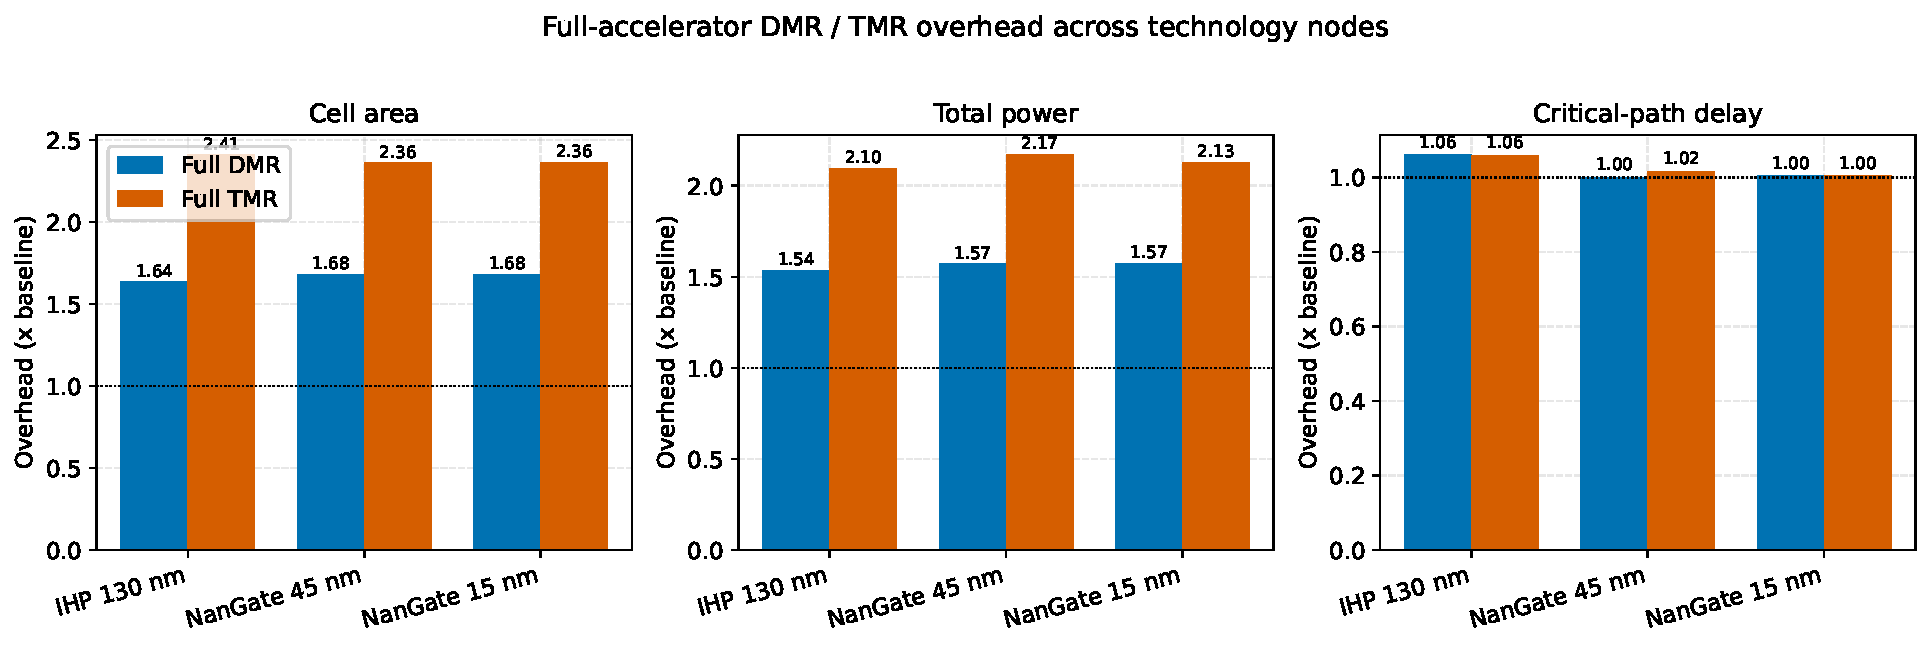
\includegraphics[width=\textwidth]{img/plots/full_overhead.pdf}
\caption{Full-accelerator DMR and TMR overhead --- area, power, and
critical-path delay --- across the three technology nodes.}
\label{fig:full}
\end{figure}

Full DMR costs about $1.64$--$1.68\times$ the baseline area and full TMR about
$2.36$--$2.41\times$, consistently across all three nodes. It is worth dwelling on why
these are \emph{below} the naive ``$2\times$ for DMR, $3\times$ for TMR''
expectation. That naive expectation would hold only if the \emph{entire} design
were duplicated or triplicated. Here, only the arithmetic functional units are
replicated; the mapping layer, the pipeline and FU controllers, the exception
unit, and the scratchpad interface remain single-copy. Since these unhardened
parts constitute a substantial fraction of the baseline, the overall multiplier
is pulled well below $2\times$ and $3\times$. This is a direct, quantitative
benefit of \emph{fine-grained} hardening: by protecting only the datapath, the
designer avoids paying to triplicate logic that may not need it.

The full-accelerator power overhead is about $1.54$--$1.57\times$ for DMR and
about $2.10$--$2.17\times$ for TMR --- still below the corresponding area factors,
for the same dilution reason as in Section~\ref{sec:res-fu}, though the gap
between the area and power penalties is narrower for the full datapath than for
any single unit, because hardening every unit activates a larger share of the
added logic.

\section{Composition of the overhead}
\label{sec:res-comp}

To understand \emph{where} the extra cost goes, Figures~\ref{fig:area-comp} and
\ref{fig:power-comp} decompose area and power by category for every Scenario~A
configuration at the mature node (the finer nodes behave analogously), and
Figure~\ref{fig:cells} shows the combinational and sequential cell counts.

\begin{figure}[htbp]
\centering
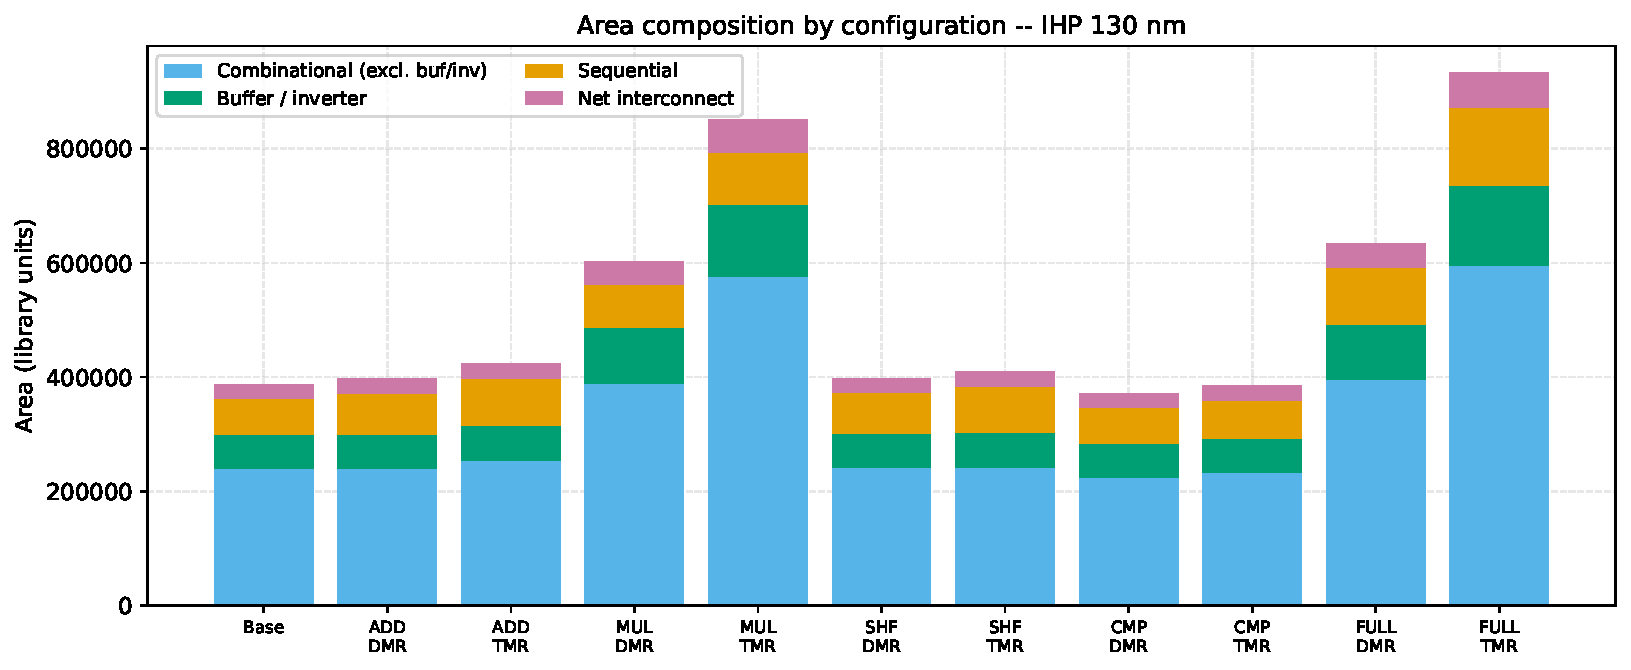
\includegraphics[width=\textwidth]{img/plots/area_composition_130nm.pdf}
\caption{Area composition by configuration at IHP 130\,nm: combinational,
buffer/inverter, sequential, and net-interconnect area. Redundancy adds
predominantly combinational logic.}
\label{fig:area-comp}
\end{figure}

\begin{figure}[htbp]
\centering
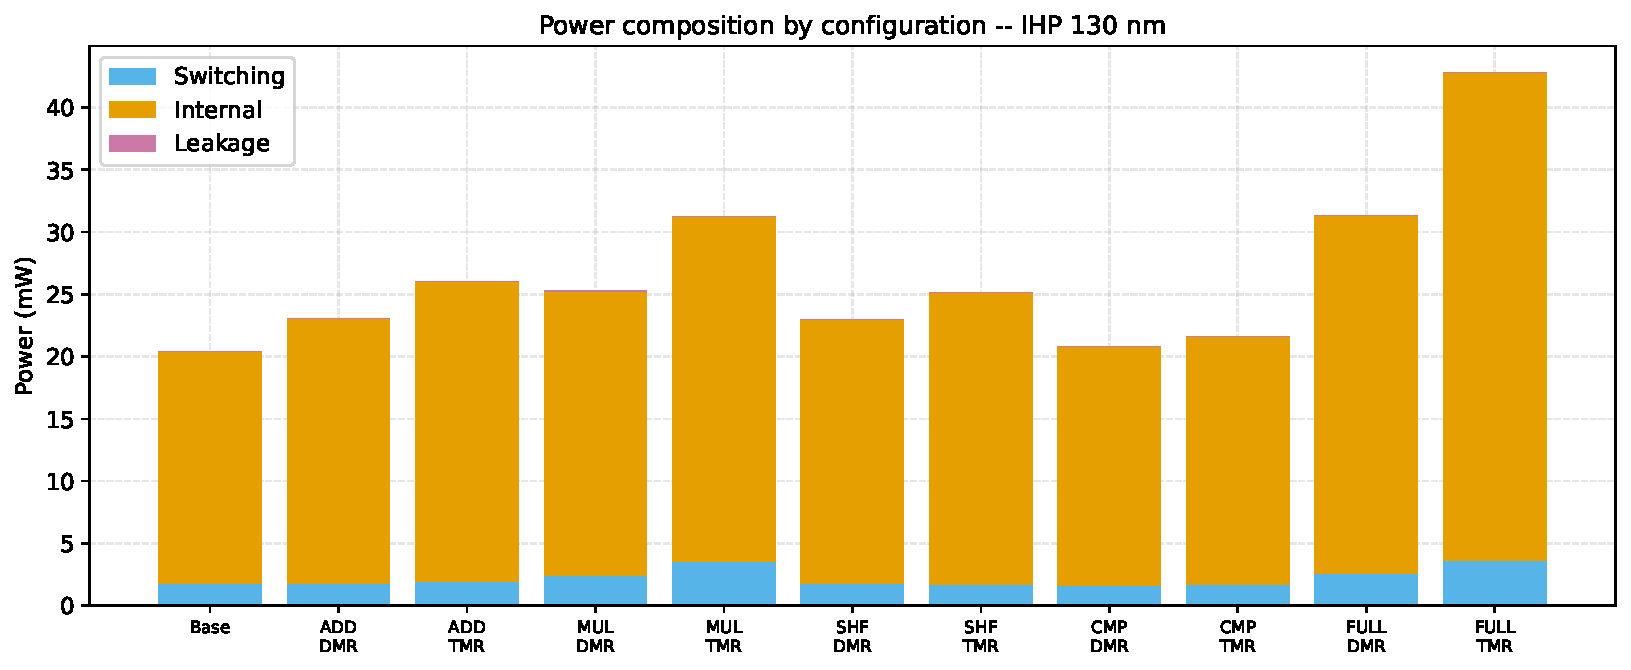
\includegraphics[width=\textwidth]{img/plots/power_composition_130nm.pdf}
\caption{Power composition by configuration at IHP 130\,nm: switching, internal,
and leakage power.}
\label{fig:power-comp}
\end{figure}

\begin{figure}[htbp]
\centering
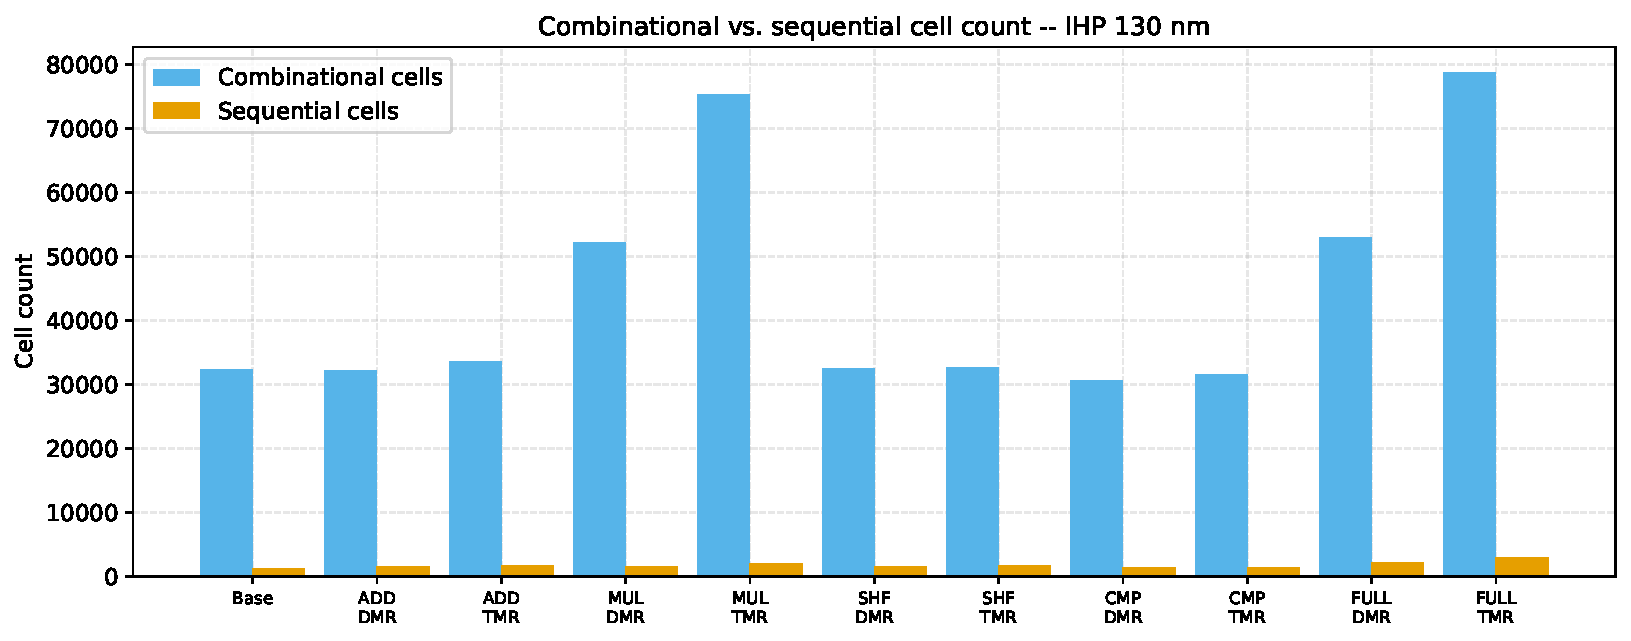
\includegraphics[width=\textwidth]{img/plots/cell_counts_130nm.pdf}
\caption{Combinational versus sequential cell counts by configuration at IHP
130\,nm. The growth is overwhelmingly in combinational cells.}
\label{fig:cells}
\end{figure}

The decomposition confirms the intuition behind the wrappers. The extra area is
overwhelmingly \emph{combinational}: the duplicated/triplicated functional-unit
logic plus the comparison/voter arrays. The sequential-cell count barely moves
for the lighter units and grows only where the protected unit is itself
pipelined and large (the multiplier). This matters for reliability reasoning:
the redundancy is concentrated exactly where transient errors in combinational
arithmetic would otherwise propagate silently. The power decomposition tells the
same story --- the increase is concentrated in the switching and internal power
of the added combinational logic, with leakage scaling roughly in proportion to
the added cells.

\subsection{Composition at the finer nodes}
\label{sec:res-comp-nodes}

The same decomposition holds at the mainstream and advanced nodes, confirming
that it reflects the structure of the redundancy rather than a quirk of one
library. Figures~\ref{fig:area-comp-45} and \ref{fig:area-comp-15} show the area
composition at NanGate 45\,nm and 15\,nm; Figures~\ref{fig:power-comp-45} and
\ref{fig:power-comp-15} the power composition; and
Figures~\ref{fig:cells-45} and \ref{fig:cells-15} the cell counts. In every case
the redundancy overhead is dominated by added combinational cells, the sequential
count grows materially only for the multiplier, and the multiplier and
full-datapath configurations stand out as the tall bars --- exactly as at the
mature node. The one systematic difference is the relative weight of leakage in
the power stacks, which grows at the finer nodes, consistent with the
well-known increase of static power in advanced CMOS; this shifts the balance of
\emph{where} the redundancy power goes but not the overall ordering of the
configurations.

\begin{figure}[htbp]
\centering
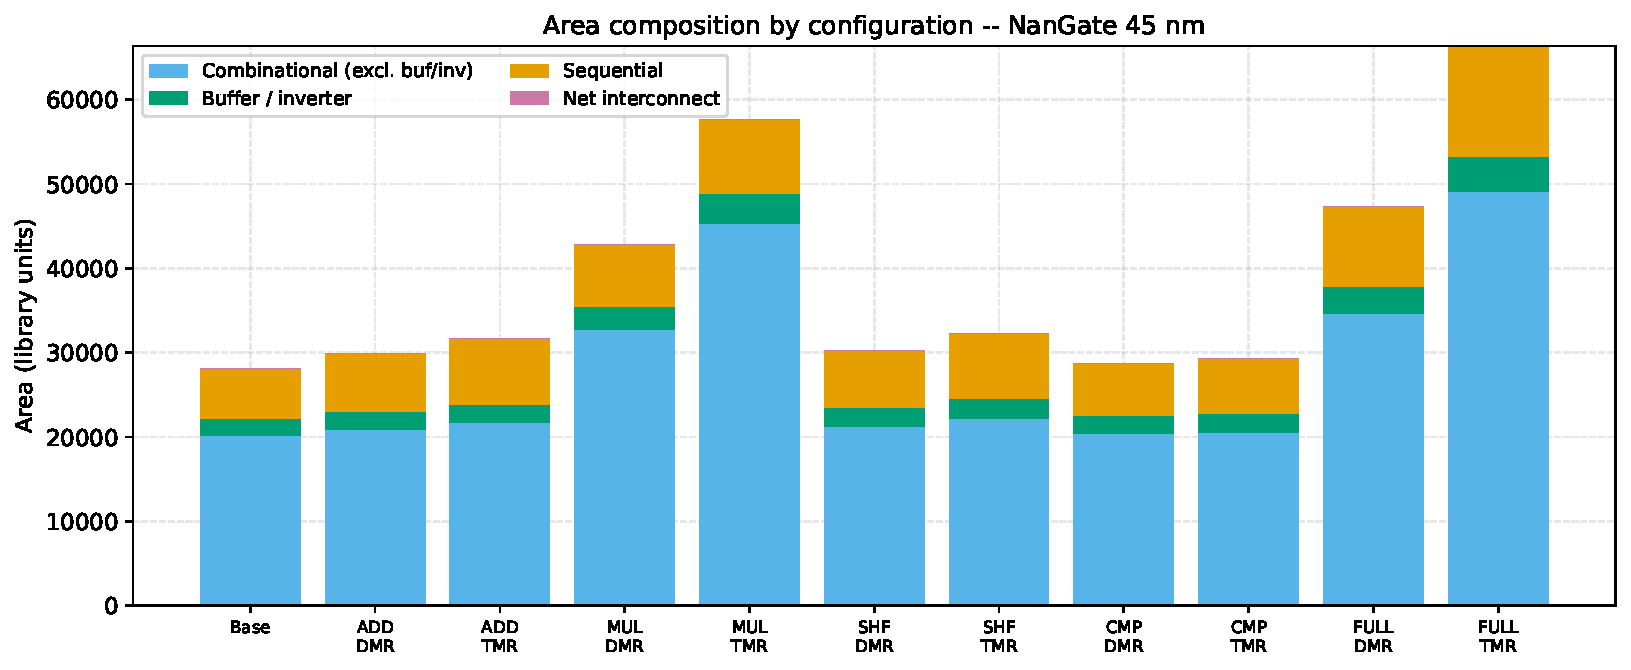
\includegraphics[width=\textwidth]{img/plots/area_composition_45nm.pdf}
\caption{Area composition by configuration at NanGate 45\,nm.}
\label{fig:area-comp-45}
\end{figure}

\begin{figure}[htbp]
\centering
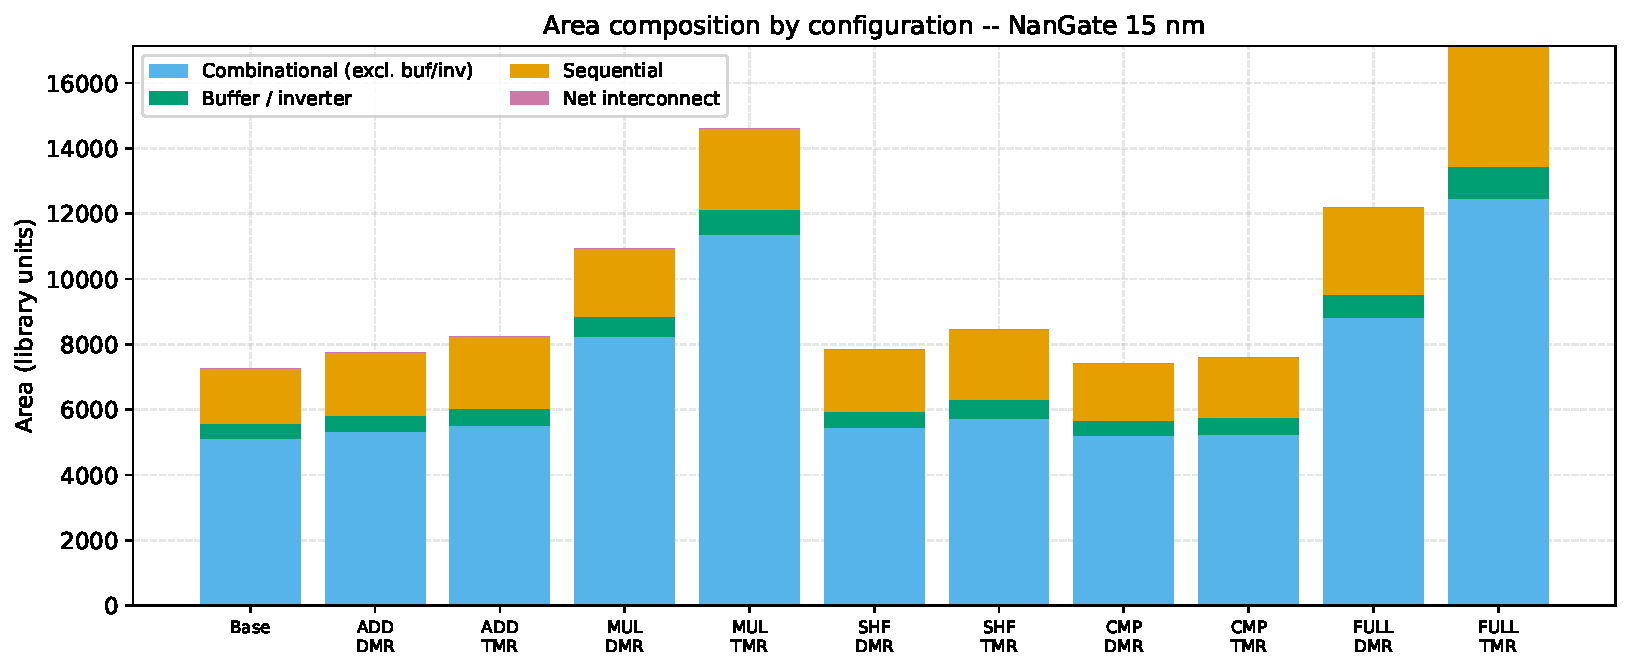
\includegraphics[width=\textwidth]{img/plots/area_composition_15nm.pdf}
\caption{Area composition by configuration at NanGate 15\,nm.}
\label{fig:area-comp-15}
\end{figure}

\begin{figure}[htbp]
\centering
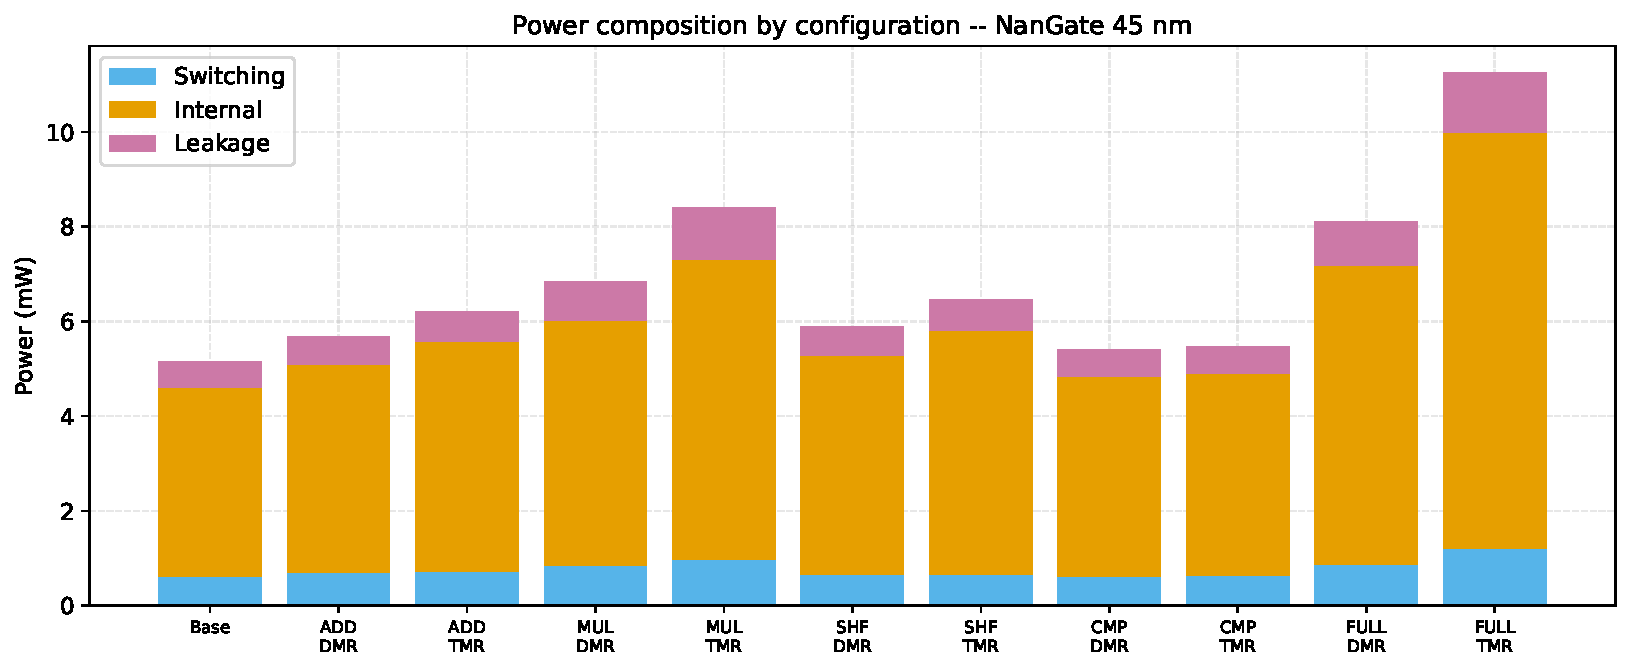
\includegraphics[width=\textwidth]{img/plots/power_composition_45nm.pdf}
\caption{Power composition by configuration at NanGate 45\,nm.}
\label{fig:power-comp-45}
\end{figure}

\begin{figure}[htbp]
\centering
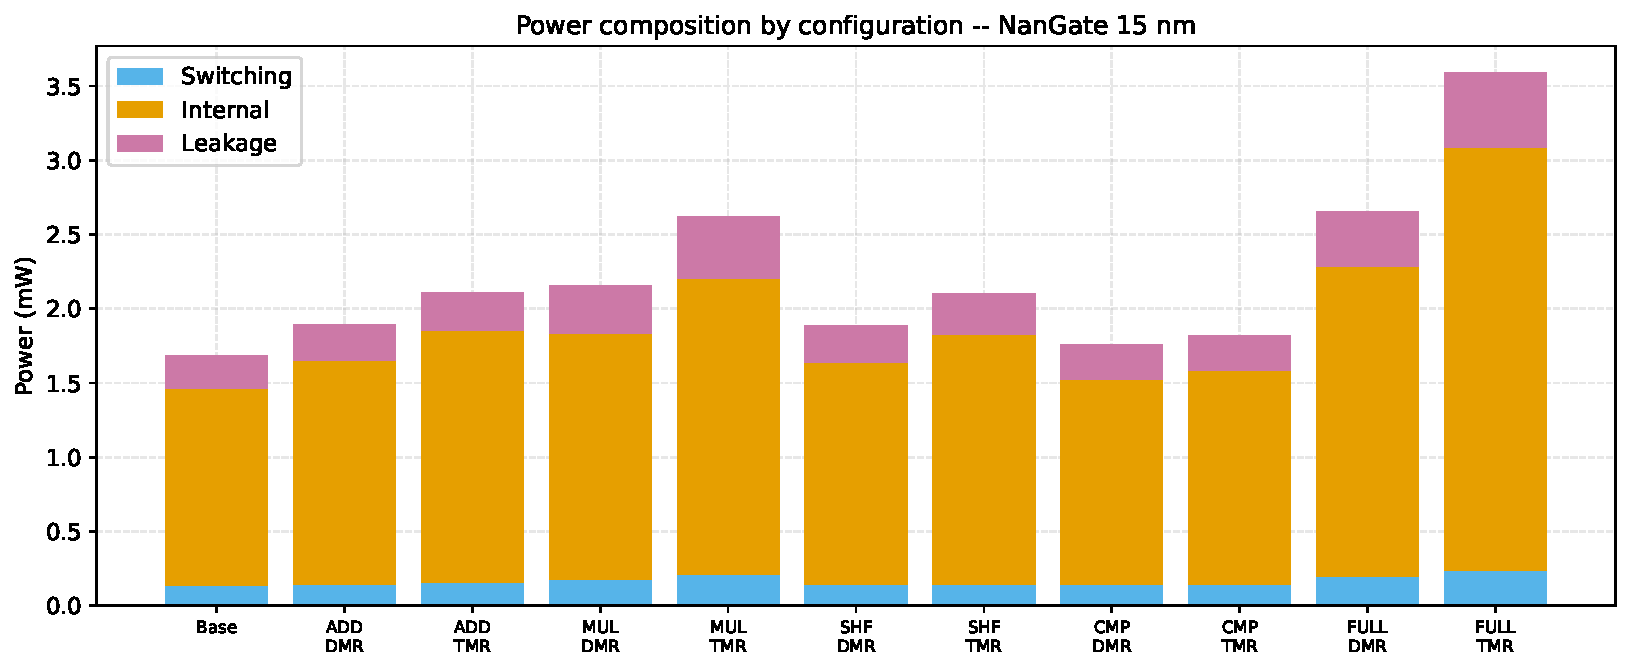
\includegraphics[width=\textwidth]{img/plots/power_composition_15nm.pdf}
\caption{Power composition by configuration at NanGate 15\,nm. Leakage takes a
visibly larger share of the total than at the mature node.}
\label{fig:power-comp-15}
\end{figure}

\begin{figure}[htbp]
\centering
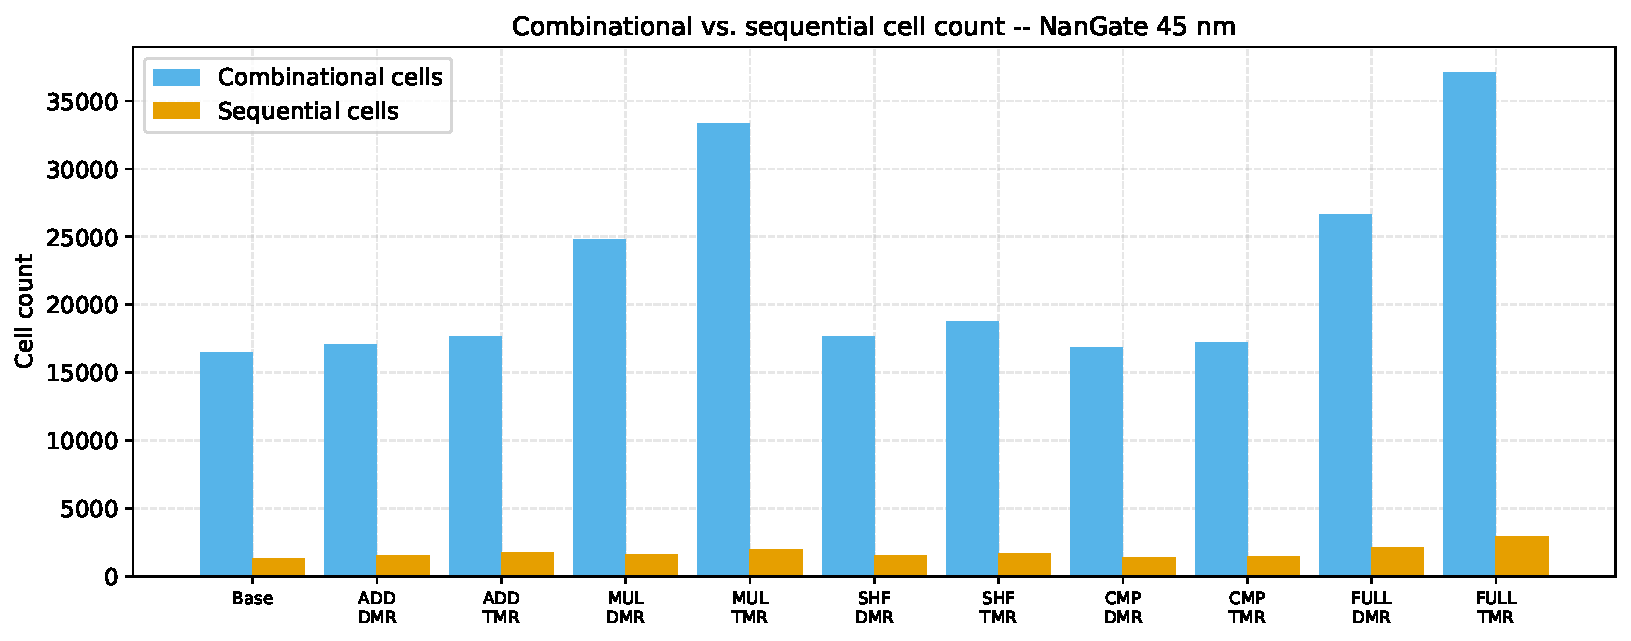
\includegraphics[width=\textwidth]{img/plots/cell_counts_45nm.pdf}
\caption{Combinational versus sequential cell counts at NanGate 45\,nm.}
\label{fig:cells-45}
\end{figure}

\begin{figure}[htbp]
\centering
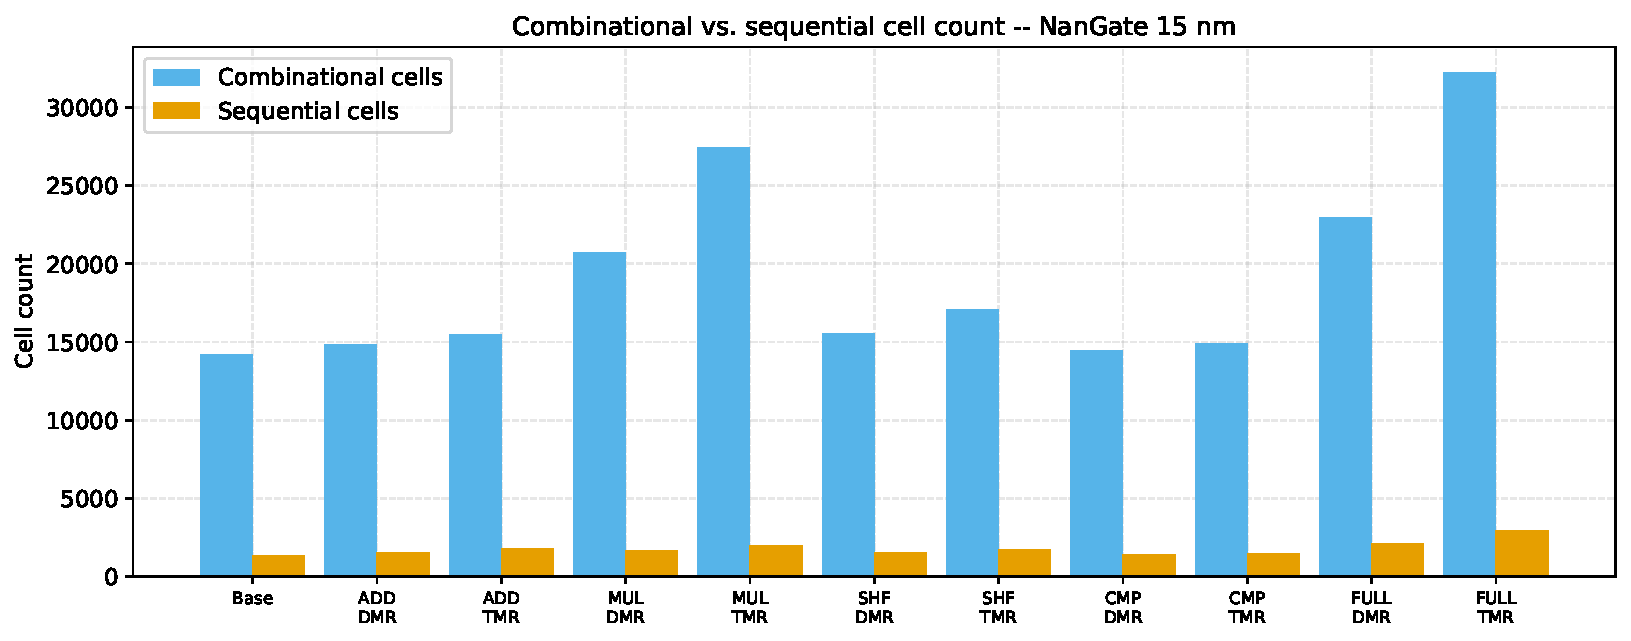
\includegraphics[width=\textwidth]{img/plots/cell_counts_15nm.pdf}
\caption{Combinational versus sequential cell counts at NanGate 15\,nm.}
\label{fig:cells-15}
\end{figure}

\section{Timing impact}
\label{sec:res-timing}

A central question for any redundancy scheme is whether it slows the design down.
The right-hand panel of Figure~\ref{fig:full} answers it: the critical-path delay
is only \emph{mildly} affected by redundancy. The overhead is largest at the
mature node --- about $1.06\times$ for both full DMR and full TMR --- and shrinks
at the finer nodes, to roughly $1.0$--$1.02\times$ at the mainstream node and
essentially $1.00\times$ at the advanced node. The per-unit delay overheads are
even smaller, and a few configurations land marginally below $1.00$, within the
noise of the timing analysis.

This is consistent with what the architecture predicts. The DMR comparator and
the TMR voter are shallow combinational layers --- a few gates deep --- placed on
the functional-unit outputs, while the accelerator's true critical path runs
through other, deeper logic (such as the address arithmetic in the
exception/control path). The voter therefore only occasionally lengthens the
critical path, and then only slightly: hardening every unit (full DMR/TMR) adds a
voter layer to more outputs and so produces the largest --- but still small ---
delay increase, most visibly at the mature node where the baseline path is
longest in absolute terms.

The practical implication is significant: across all three nodes, \emph{the
designer buys fault tolerance with area and power at a delay cost of at most a
few percent}, which removes one of the usual objections to modular redundancy in
high-throughput datapaths.

\section{Area--power trade-off}
\label{sec:res-tradeoff}

Figure~\ref{fig:tradeoff} plots, for the mature node, every Scenario~A
configuration in the area-overhead/power-overhead plane. The configurations form
a clear frontier from the cheap comparator points near the baseline, through the
adder and shifter, to the expensive multiplier and full-datapath points. DMR
points (squares) always sit below and to the left of the corresponding TMR points
(triangles): DMR delivers detection at roughly half the marginal cost of the
masking that TMR provides. The figure is a compact decision aid --- a designer
with a fixed area or power budget can read off which units can be afforded.

\begin{figure}[htbp]
\centering
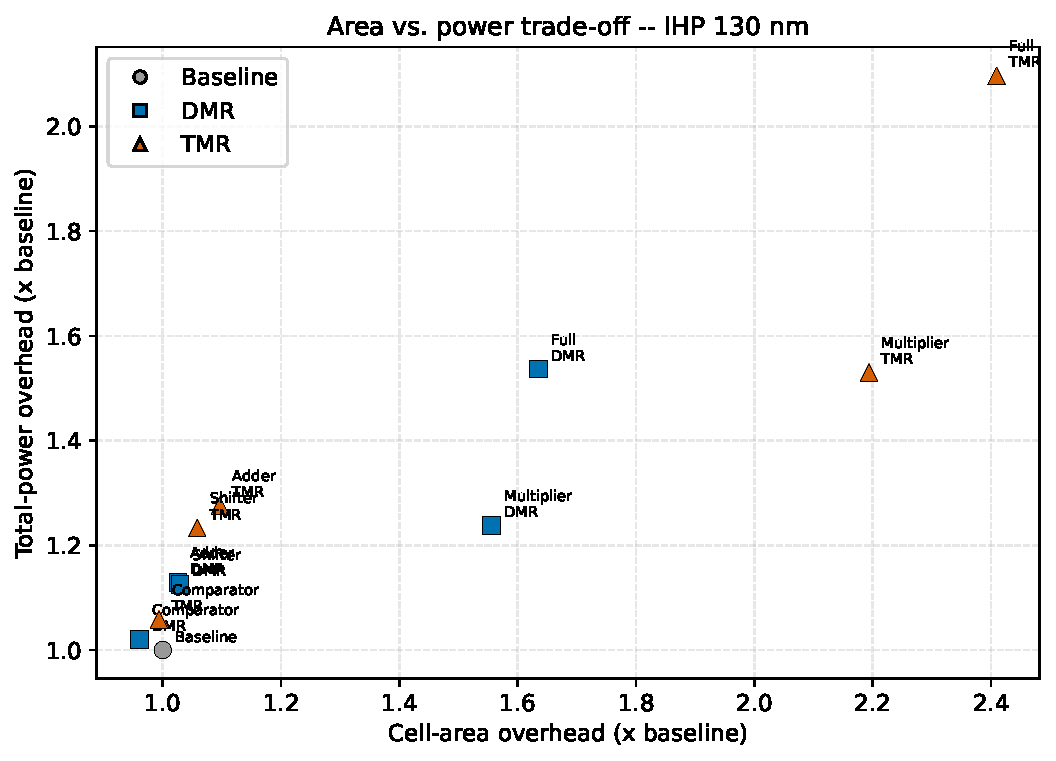
\includegraphics[width=0.78\textwidth]{img/plots/tradeoff_130nm.pdf}
\caption{Area versus power overhead for every single-core configuration at IHP
130\,nm. DMR (squares) consistently dominates TMR (triangles) in cost; the
multiplier and full-datapath points define the expensive end of the frontier.}
\label{fig:tradeoff}
\end{figure}

The same frontier reappears at the other two nodes
(Figures~\ref{fig:tradeoff-45} and \ref{fig:tradeoff-15}): although the absolute
power and area scales differ, the \emph{shape} of the trade-off --- comparator
cheapest, multiplier and full datapath most expensive, DMR dominating TMR --- is
preserved, reinforcing that the decision aid is technology-independent.

\begin{figure}[htbp]
\centering
\begin{subfigure}[t]{0.49\textwidth}
\centering
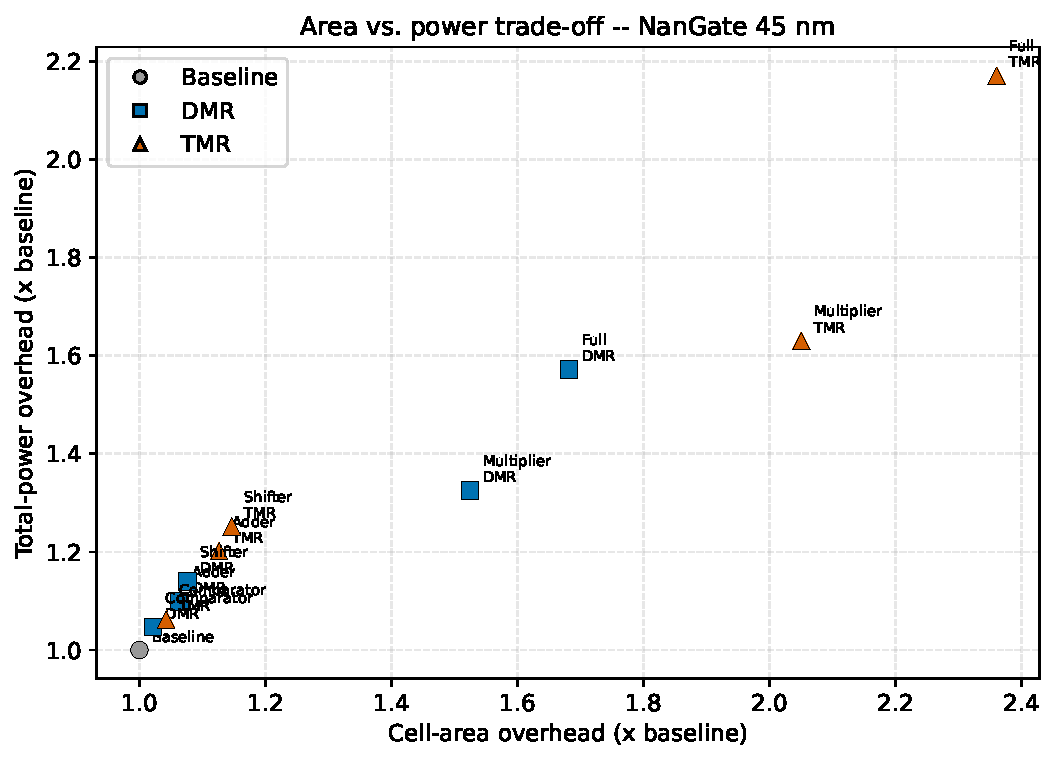
\includegraphics[width=\textwidth]{img/plots/tradeoff_45nm.pdf}
\caption{NanGate 45\,nm.}
\label{fig:tradeoff-45}
\end{subfigure}
\hfill
\begin{subfigure}[t]{0.49\textwidth}
\centering
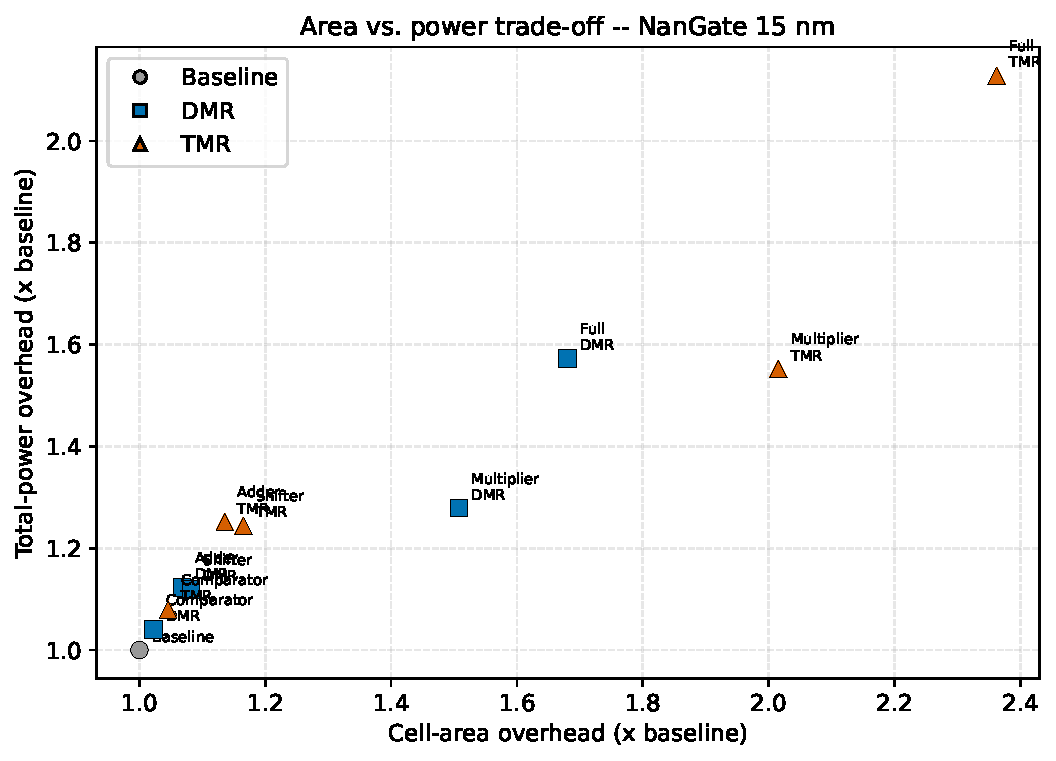
\includegraphics[width=\textwidth]{img/plots/tradeoff_15nm.pdf}
\caption{NanGate 15\,nm.}
\label{fig:tradeoff-15}
\end{subfigure}
\caption{Area versus power trade-off at the mainstream and advanced nodes. The
frontier has the same shape as at the mature node (Figure~\ref{fig:tradeoff}).}
\label{fig:tradeoff-fine}
\end{figure}

The absolute cell areas behind these ratios are shown, per node, in
Figure~\ref{fig:abs-area}; the shapes are identical across nodes even though the
vertical scales differ by orders of magnitude, which is the clearest possible
demonstration that the \emph{relative} cost structure is a property of the
architecture rather than of any one technology.

\begin{figure}[htbp]
\centering
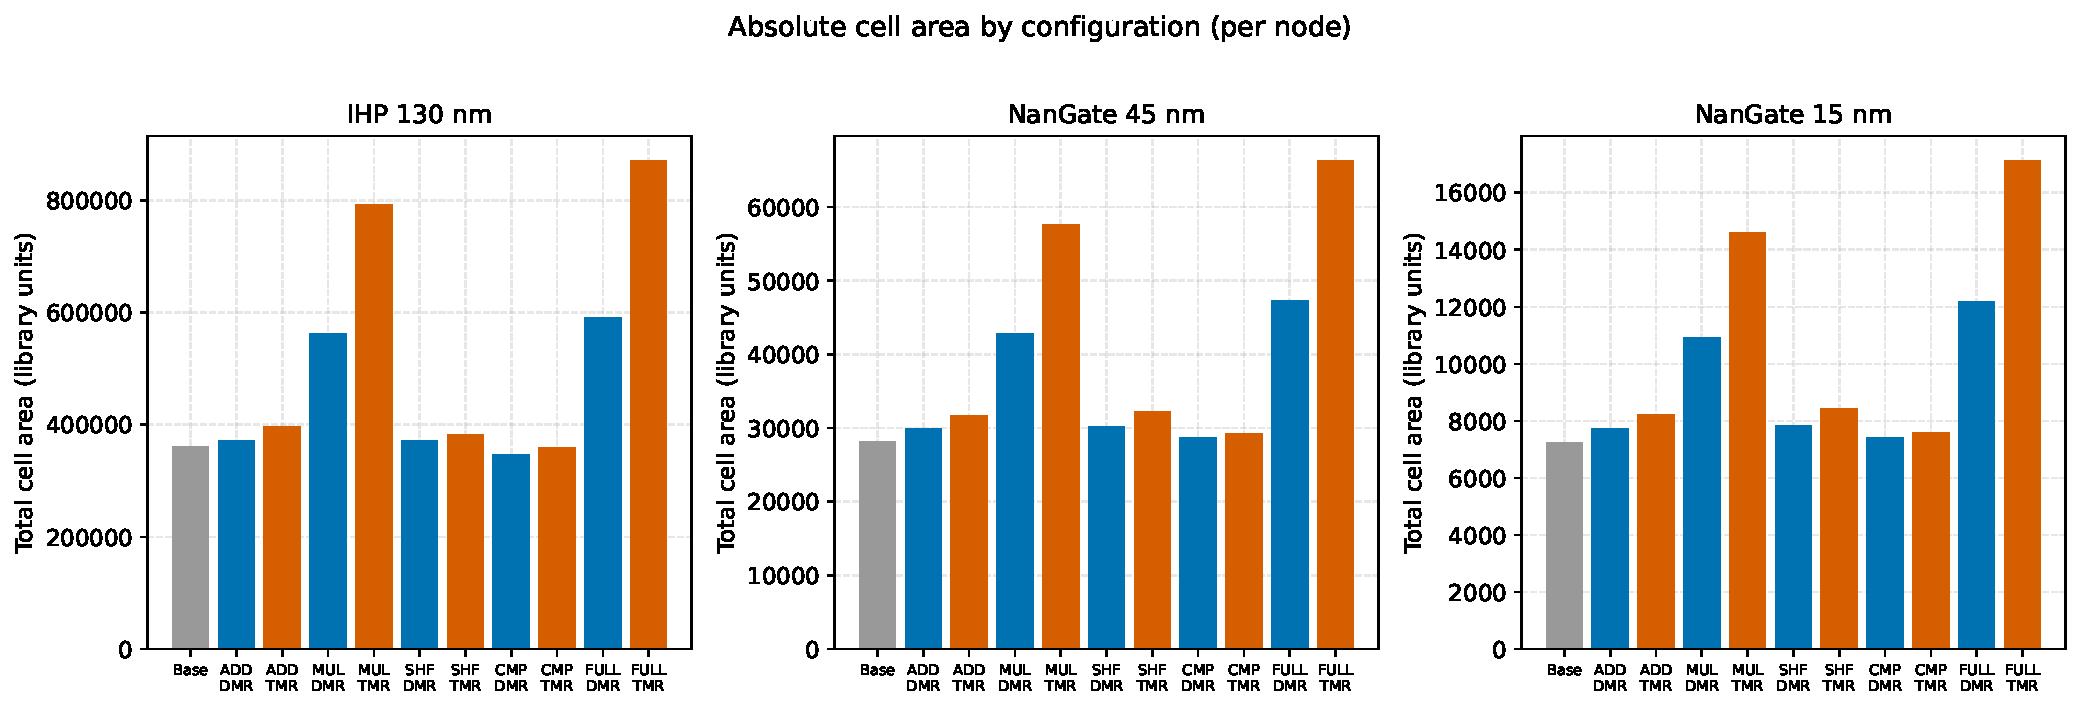
\includegraphics[width=\textwidth]{img/plots/absolute_area.pdf}
\caption{Absolute total cell area by configuration at each node (note the
differing vertical scales). The relative pattern is invariant across nodes.}
\label{fig:abs-area}
\end{figure}

\section{Replication-based redundancy}
\label{sec:res-repl}

Scenario~B evaluates the alternative regime in which the accelerator is already
replicated into three lanes for throughput, and redundancy is obtained by voting
the lanes in the mapping layer. Table~\ref{tab:replication} and
Figure~\ref{fig:repl} report the results.

\begin{table}[htbp]
\centering
\caption{Replication-based redundancy (Scenario~B): three-lane accelerator with voting inserted in the mapping unit. Cell area is given in library units and also normalised to the single-core baseline. Adding voting changes the area only marginally relative to the replicated baseline.}
\label{tab:replication}
\small
\begin{tabular}{llrr}
\toprule
Node & Configuration & Cell area & $\times$ single-core \\
\midrule
IHP 130\,nm & Replicated baseline (3 lanes) & 1,011,568 & 2.80 \\
IHP 130\,nm & Replicated + DMR voting & 950,085 & 2.63 \\
IHP 130\,nm & Replicated + TMR voting & 938,713 & 2.60 \\
\midrule
NanGate 45\,nm & Replicated baseline (3 lanes) & 84,179 & 2.99 \\
NanGate 45\,nm & Replicated + DMR voting & 84,401 & 3.00 \\
NanGate 45\,nm & Replicated + TMR voting & 84,315 & 3.00 \\
\midrule
NanGate 15\,nm & Replicated baseline (3 lanes) & 21,752 & 3.00 \\
NanGate 15\,nm & Replicated + DMR voting & 21,954 & 3.03 \\
NanGate 15\,nm & Replicated + TMR voting & 22,161 & 3.06 \\
\bottomrule
\end{tabular}
\end{table}


\begin{figure}[htbp]
\centering
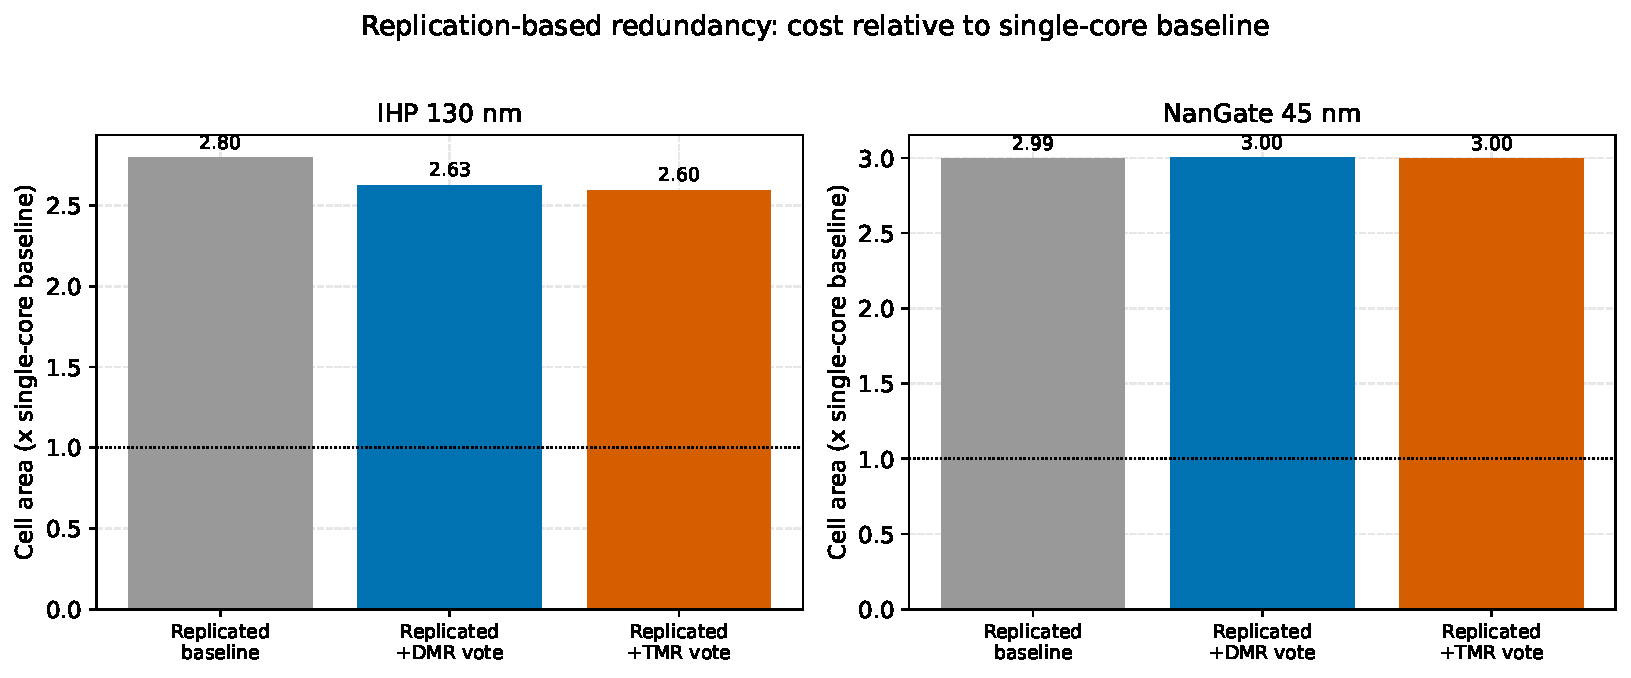
\includegraphics[width=\textwidth]{img/plots/replication_area.pdf}
\caption{Cost of replication-based redundancy relative to the single-core
baseline. The three-lane datapath itself costs roughly $3\times$; adding DMR or
TMR voting on top of it changes the area only marginally.}
\label{fig:repl}
\end{figure}

Two facts stand out. First, the replicated baseline already costs about
$2.8$--$3.0\times$ the single-core baseline --- essentially the unavoidable price
of three lanes. Second, and more interestingly, \emph{adding voting on top of
replication is almost free}: at the mainstream node the replicated-plus-DMR and
replicated-plus-TMR areas sit within a fraction of a percent of the replicated
baseline, and at the advanced node they add only about one to two percent. At the
mature node the voting variants even synthesise slightly \emph{smaller} than the
plain replicated baseline ($2.60$--$2.63\times$ versus $2.80\times$), which is a
clear sign that the marginal logic added by voting is below the noise floor of
synthesis optimisation --- the optimiser simply restructures the large replicated
datapath differently between runs. In every case the message is the same: because
the expensive datapath copies already exist for throughput, only the thin
comparison/voter logic in the mapping layer is genuinely new. The lesson is that
the economics of redundancy depend strongly on context: building TMR from scratch
costs about $2.4\times$ (Section~\ref{sec:res-full}), but \emph{reusing}
replication that is already present for performance turns masking into a
negligible add-on.

\section{Stability across technology nodes}
\label{sec:res-nodes}

Table~\ref{tab:overhead} collects the area and power overheads of every
single-core configuration at all three nodes side by side, and
Figure~\ref{fig:node-summary} tracks the full-accelerator overheads across nodes.

\begin{table}[htbp]
\centering
\caption{Cell-area and total-power overhead of each single-core fault-tolerance configuration, normalised to the per-node baseline ($\times$ baseline). Values are remarkably stable across the three technology nodes.}
\label{tab:overhead}
\small
\begin{tabular}{lrrrrrr}
\toprule
 & \multicolumn{2}{c}{IHP 130\,nm} & \multicolumn{2}{c}{NanGate 45\,nm} & \multicolumn{2}{c}{NanGate 15\,nm} \\
\cmidrule(lr){2-3} \cmidrule(lr){4-5} \cmidrule(lr){6-7}
Configuration & Area & Power & Area & Power & Area & Power \\
\midrule
Adder DMR & 1.03 & 1.13 & 1.06 & 1.10 & 1.07 & 1.12 \\
Adder TMR & 1.10 & 1.28 & 1.13 & 1.20 & 1.14 & 1.25 \\
Multiplier DMR & 1.56 & 1.24 & 1.52 & 1.33 & 1.51 & 1.28 \\
Multiplier TMR & 2.19 & 1.53 & 2.05 & 1.63 & 2.02 & 1.55 \\
Shifter DMR & 1.03 & 1.13 & 1.08 & 1.14 & 1.08 & 1.12 \\
Shifter TMR & 1.06 & 1.23 & 1.15 & 1.25 & 1.17 & 1.24 \\
Comparator DMR & 0.96 & 1.02 & 1.02 & 1.05 & 1.02 & 1.04 \\
Comparator TMR & 0.99 & 1.06 & 1.04 & 1.06 & 1.05 & 1.08 \\
Full DMR & 1.64 & 1.54 & 1.68 & 1.57 & 1.68 & 1.57 \\
Full TMR & 2.41 & 2.10 & 2.36 & 2.17 & 2.36 & 2.13 \\
\bottomrule
\end{tabular}
\end{table}


\begin{figure}[htbp]
\centering
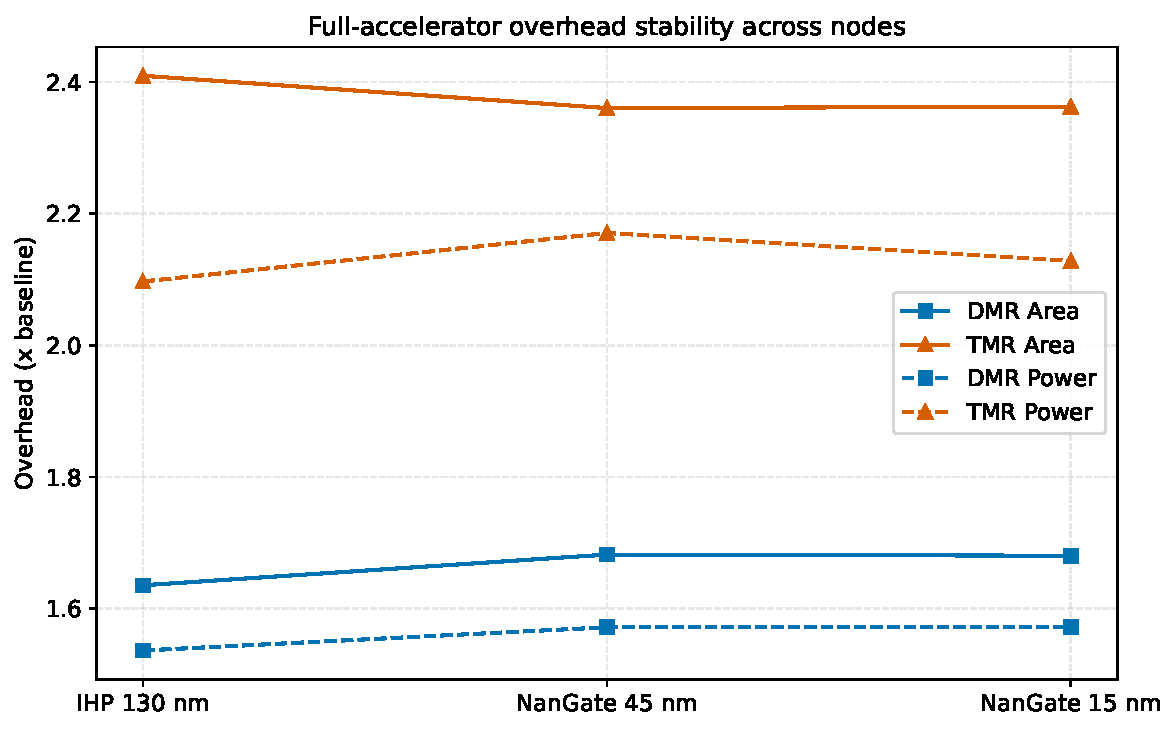
\includegraphics[width=0.72\textwidth]{img/plots/node_summary.pdf}
\caption{Full-accelerator area and power overheads tracked across the three
nodes. The lines are almost flat, showing that the cost of redundancy is a
stable architectural property.}
\label{fig:node-summary}
\end{figure}

The overheads are remarkably consistent: the area factors vary by at most a few
percent across a technology range spanning from 130\,nm down to 15\,nm. This
stability is the second major result of the study. It means that the design
guidelines derived here are not tied to a particular library: a designer can
estimate the cost of a given hardening choice on a new node directly from these
factors, with confidence that the architecture-level ratios will carry over. The
small deviations that do appear --- chiefly the slightly higher power and delay
overheads at the advanced node --- are consistent with the finer node's more
balanced cell/wire delays and its different leakage profile, and do not change
the qualitative picture.

\section{Design guidelines}
\label{sec:res-guidelines}

The results support a compact set of guidelines for hardening a SIMD vector
accelerator of this kind:

\begin{enumerate}
  \item \textbf{Spend the budget on the multiplier last, the comparator first.}
        Because the multiplier dominates the cost of any scheme that includes it,
        and the comparator is almost free, a graceful hardening path is to
        protect the cheap units first and add multiplier protection only when the
        reliability requirement justifies its large area cost.
  \item \textbf{Use DMR for detection, TMR for masking, and choose by system
        need.} DMR roughly halves the marginal cost of TMR while still catching
        errors; if the system can respond to an error flag (retry, rollback, safe
        state), DMR is the economical choice. Reserve TMR for units whose output
        must remain correct without interruption.
  \item \textbf{Harden at fine granularity to avoid over-paying.} Full-datapath
        TMR costs about $2.4\times$ rather than $3\times$ precisely because the
        non-datapath logic is left single-copy; selective hardening lets the
        designer push this saving further.
  \item \textbf{Exploit existing replication.} If the accelerator is already
        replicated for throughput, obtain reliability by voting the existing
        lanes --- the marginal cost is small compared with building redundancy
        anew.
  \item \textbf{Add in-field monitoring freely.} The IJTAG instrumentation costs
        at most a couple of percent (Chapter~\ref{ch:ijtag}) and is independent
        of the redundancy choice, so observability can be combined with any
        hardening configuration without materially changing its cost.
  \item \textbf{Trust the ratios across nodes.} The overhead factors are stable
        across the studied process range, so they can be reused to estimate cost
        on other nodes.
\end{enumerate}

\chapter{Conclusions and Future Work}
\label{ch:conclusion}

\section{Summary}

This thesis set out to make the SIMD vector accelerator of the Klessydra RISC-V
architecture both \emph{fault-tolerant} and \emph{observable in the field}, and
to do so in a way that is reusable and automatable rather than bespoke. Three
contributions delivered on that goal.

First, the originally monolithic accelerator was \emph{re-engineered into a clean
modular hierarchy} in which each functional unit --- adder, multiplier, shifter,
comparator, and accumulator --- is an independently instantiable VHDL entity with
an explicit interface. This restructuring is the enabling substrate for
everything that follows: it is what allows redundancy and instrumentation to be
attached at arbitrary granularity without disturbing the surrounding logic.

Second, a \emph{reusable fault-tolerance framework} was built on top of this
structure from two tiny, technology-independent primitives --- a DMR comparison
cell that provides error detection through an error flag, and a TMR majority
voter that provides error masking. Wrapping the functional units with these
primitives produced a complete family of hardened configurations: each unit
hardened individually, the full datapath hardened together, and an alternative
replication-based scheme that votes already-existing parallel lanes.

Third, an \emph{automated IEEE~1687 (IJTAG) instrumentation flow} was developed
that inserts on-chip sensors into the VHDL hierarchy from pragma markers and a
single JSON description, and generates the Tessent scripts that extract the
instrument connectivity and build the hierarchical access network with Segment
Insertion Bits --- giving in-field observability with no manual rewiring.

Finally, every configuration was synthesised across three technology nodes
spanning a mature, a mainstream, and an advanced process, and the resulting data
were reduced to a consistent set of comparisons. The exploration produced several
clear and actionable findings:

\begin{itemize}
  \item The cost of redundancy is dominated by \emph{which} functional unit is
        hardened: the multiplier is by far the most expensive and the comparator
        almost free, so fine-grained, selective hardening is highly effective.
  \item Hardening only the datapath keeps full-accelerator DMR and TMR well below
        the naive $2\times$ and $3\times$ factors, because the control, mapping,
        and memory-interface logic remain single-copy.
  \item Redundancy adds area and power but only a few percent of critical-path
        delay (at most about $1.06\times$, at the mature node), because the
        comparators and voters are shallow layers that rarely sit on the
        critical path.
  \item When the accelerator is already replicated for throughput, adding voting
        on top is nearly free in area --- redundancy economics are
        context-dependent.
  \item The in-field monitoring instrumentation costs at most a couple of percent
        and is independent of the redundancy choice.
  \item All of these overhead factors are \emph{stable across the technology
        range}, so the resulting design guidelines transfer between nodes.
\end{itemize}

Together, these results constitute a reusable, automatable methodology for
hardening a RISC-V vector accelerator against faults while keeping it observable
in the field, accompanied by quantitative guidelines for navigating the
protection-versus-cost trade-off.

\section{Limitations}

Several limitations should be kept in mind when interpreting the results. The
power figures are estimates from default switching activity rather than from
gate-level activity captured on representative workloads, so they are most
meaningful as ratios. Timing was characterised against a single aggressive clock
target that no configuration meets, so the comparison rests on relative
critical-path (data-arrival) delays rather than on closing timing at a realistic
frequency. The fault-tolerance claims are \emph{structural}:
DMR detects and TMR masks any single discrepancy by construction, but the study
did not run an explicit fault-injection campaign to measure the resulting
reduction in failure rate. Finally, the advanced-node replication runs collapsed
to an identical netlist and were therefore not over-interpreted.

\section{Future work}

The framework opens several natural directions.

\begin{itemize}
  \item \textbf{Fault-injection validation.} Coupling the hardened
        configurations with an RTL or gate-level fault-injection campaign would
        turn the structural guarantees into measured reliability metrics (e.g.,
        architectural vulnerability factor and failures-in-time), and would let
        selective-hardening decisions be guided by measured per-unit
        vulnerability rather than area alone.
  \item \textbf{Constrained and gate-level-activity synthesis.} Repeating the
        sweep with binding clock constraints and workload-derived switching
        activity would refine the power and timing figures and reveal any
        frequency penalty at aggressive targets.
  \item \textbf{Richer redundancy.} Triplicated voters for the most critical
        outputs, residue or parity checking for the multiplier, and selective
        ECC on the scratchpad would broaden the protection palette and could be
        evaluated within the same modular structure.
  \item \textbf{Closed-loop monitoring.} The IJTAG activity and thermal sensors
        could drive run-time adaptation --- throttling, voltage/frequency
        scaling, or reconfiguration of the redundancy mode --- turning passive
        observability into active in-field health management. Adding further
        sensor types (thermal, ageing, voltage) to the existing tool is
        straightforward given its sensor-agnostic interface.
  \item \textbf{Broader design space.} Sweeping the SIMD width and lane count
        together with the redundancy options would map how the cost structure
        scales with accelerator size, and extending the flow to other Klessydra
        cores or to other RISC-V accelerators would test the generality of the
        methodology.
\end{itemize}

In bringing structural redundancy and standardised in-field monitoring together
on one parameterised RISC-V vector accelerator, and characterising the result
across three technology nodes, this thesis provides both a practical toolset and
an empirical foundation for designing dependable RISC-V acceleration in
safety- and mission-critical systems.


\appendix
\chapter{Tooling and Reproducibility}
\label{app:tools}

This appendix documents the data-reduction and figure-generation tooling that
turns the raw Design Compiler reports into the tables and figures of
Chapter~\ref{ch:results}, so that the results are fully reproducible. The
complete source --- the modular accelerator, the DMR/TMR wrappers, the IJTAG
sensor-insertion tool, and the synthesis-sweep and data-reduction scripts ---
together with the thesis sources is available in the project repository at
\href{\repourl}{\repourl}.

\section{Directory layout}

The synthesis reports are organised by node and configuration:
\begin{itemize}
  \item \texttt{synth\_output/<node>/<config>/Report\_*.txt} --- the per-run
        area, cells, power, timing, references, and resources reports for the
        redundancy study (Scenarios A and B).
  \item \texttt{modules/out/<n>sensor/synthesis\_reports\_*/} --- the area, cells,
        power, and references reports for the IJTAG-instrumented builds, in
        \emph{counted} and \emph{black-box} accounting modes.
\end{itemize}

\section{Data-reduction scripts}

Three Python scripts perform the reduction; all are pure-Python plus
\texttt{matplotlib}/\texttt{numpy} and write into \texttt{thesis/data/} and
\texttt{thesis/img/plots/}:

\begin{itemize}
  \item \texttt{parse\_synth.py} --- parses every redundancy-study report,
        normalises power units to milliwatts, maps the on-disk configuration
        names to clean keys, and emits \texttt{synth\_data.csv} and a
        baseline-normalised \texttt{overhead\_scenarioB.csv}.
  \item \texttt{parse\_ijtag.py} --- parses the instrumented builds and emits
        \texttt{ijtag\_data.csv} and the counted-minus-black-box
        \texttt{ijtag\_cost.csv}.
  \item \texttt{make\_plots.py} and \texttt{make\_tables.py} --- generate every
        figure (as vector PDF) and every booktabs table directly from the CSVs.
\end{itemize}

Re-running the four scripts regenerates all numerical content of the thesis from
the raw reports. Listing~\ref{lst:power-parse} shows the core of the
unit-normalisation logic, which reads the power unit from each report header so
that the milliwatt/microwatt and picowatt/nanowatt differences between libraries
are reconciled automatically.

\begin{lstlisting}[language=mypython, caption={Power-unit normalisation in \texttt{parse\_synth.py} (excerpt).}, label={lst:power-parse}]
for ln in lines:
    m = re.search(r"Dynamic Power Units = 1(\w?)W", ln)
    if m:
        u = m.group(1)
        dyn_scale = {"m":1.0,"u":1e-3,"n":1e-6,"p":1e-9,"":1e3}.get(u, 1.0)
    m = re.search(r"Leakage Power Units = 1(\w?)W", ln)
    if m:
        u = m.group(1)
        leak_scale = {"m":1.0,"u":1e-3,"n":1e-6,"p":1e-9,"":1e3}.get(u, 1.0)
# top-of-hierarchy row holds the whole-design power (switch, int, leak, total)
\end{lstlisting}

\chapter{Configuration Reference}
\label{app:config}

\section{Redundancy enable constants (Scenario A)}

In the single-core flow the top-level design exposes the Boolean constants
\texttt{ADDERS\_DMR\_EN}, \texttt{ADDERS\_TMR\_EN}, \texttt{MULTIPLIERS\_DMR\_EN},
\texttt{MULTIPLIERS\_TMR\_EN}, \texttt{SHIFTERS\_DMR\_EN},
\texttt{SHIFTERS\_TMR\_EN}, \texttt{COMPARATORS\_DMR\_EN}, and
\texttt{COMPARATORS\_TMR\_EN}. Setting exactly one DMR/TMR constant true gives a
single-FU configuration; setting all four DMR (or all four TMR) constants true
gives full DMR (or full TMR); leaving all false gives the baseline.

\section{Replication constants (Scenario B)}

In the replicated flow, \texttt{replicate\_accl\_en} is enabled
(\texttt{ACCL\_NUM} = \texttt{FU\_NUM} = 3) and the redundancy lives in the
mapping layer, toggled by its \texttt{DMR\_ENABLED} and \texttt{TMR\_ENABLED}
constants: neither set gives the replicated baseline, \texttt{DMR\_ENABLED} gives
replicated-plus-DMR, and \texttt{TMR\_ENABLED} gives replicated-plus-TMR.

\section{IJTAG sensor configuration}

The IJTAG flow is driven by a single \texttt{config.json} that declares the
top-level entity, clock, libraries, packages, the activity-sensor type with its
ICL client-port names, and the sensor instances with their generic maps
(\texttt{SENSOR\_ID}, \texttt{WINDOW\_WIDTH}), functional port maps, and
hierarchical paths. The \texttt{configurations} section groups instances into the
cumulative \texttt{1sensor}/\texttt{2sensor}/\texttt{3sensor} builds used in
Section~\ref{sec:ij-synth}.


\cleardoublepage
\addcontentsline{toc}{chapter}{Bibliography}
\begin{thebibliography}{99}
\bibitem{riscv-isa}
A.~Waterman and K.~Asanovi\'c (eds.),
``The RISC-V Instruction Set Manual, Volume I: Unprivileged ISA,''
RISC-V International, 2019.

\bibitem{riscv-vector}
RISC-V International,
``RISC-V ``V'' Vector Extension Specification,'' 2021.

\bibitem{klessydra}
M.~Olivieri, A.~Cheikh, G.~Cerutti, A.~Mastrandrea, and F.~Menichelli,
``Investigation on the optimal pipeline organization in RISC-V multi-threaded
soft processor cores,'' in \emph{IEEE Int. System-on-Chip Conf. (SOCC)}, 2017.

\bibitem{klessydra-dsp}
A.~Cheikh, G.~Cerutti, A.~Mastrandrea, F.~Menichelli, and M.~Olivieri,
``The microarchitecture of a multi-threaded RISC-V compliant processing core
family for IoT end-nodes,'' in \emph{Applications in Electronics Pervading
Industry, Environment and Society (ApplePies)}, 2019.

\bibitem{vonneumann}
J.~von Neumann,
``Probabilistic logics and the synthesis of reliable organisms from unreliable
components,'' in \emph{Automata Studies}, Princeton Univ. Press, 1956.

\bibitem{koren}
I.~Koren and C.~M.~Krishna,
\emph{Fault-Tolerant Systems}, 2nd ed. Morgan Kaufmann, 2020.

\bibitem{siewiorek}
D.~P.~Siewiorek and R.~S.~Swarz,
\emph{Reliable Computer Systems: Design and Evaluation}, 3rd ed. A K Peters, 1998.

\bibitem{avizienis}
A.~Aviz\^ienis, J.-C.~Laprie, B.~Randell, and C.~Landwehr,
``Basic concepts and taxonomy of dependable and secure computing,''
\emph{IEEE Trans. Dependable Secure Comput.}, vol.~1, no.~1, pp.~11--33, 2004.

\bibitem{baumann}
R.~C.~Baumann,
``Radiation-induced soft errors in advanced semiconductor technologies,''
\emph{IEEE Trans. Device Mater. Rel.}, vol.~5, no.~3, pp.~305--316, 2005.

\bibitem{mukherjee}
S.~S.~Mukherjee, C.~Weaver, J.~Emer, S.~K.~Reinhardt, and T.~Austin,
``A systematic methodology to compute the architectural vulnerability factors
for a high-performance microprocessor,'' in \emph{36th Int. Symp.
Microarchitecture (MICRO)}, 2003.

\bibitem{nicolaidis}
M.~Nicolaidis,
``Time redundancy based soft-error tolerance to rescue nanometer technologies,''
in \emph{17th IEEE VLSI Test Symp.}, 1999.

\bibitem{tmr-fpga}
F.~L.~Kastensmidt, L.~Carro, and R.~Reis,
\emph{Fault-Tolerance Techniques for SRAM-Based FPGAs}. Springer, 2006.

\bibitem{lockstep}
X.~Iturbe, B.~Venu, E.~Ozer, and S.~Das,
``A triple core lock-step (TCLS) ARM Cortex-R5 processor for safety-critical and
ultra-reliable applications,'' in \emph{46th Annual IEEE/IFIP Int. Conf. on
Dependable Systems and Networks Workshop (DSN-W)}, 2016.

\bibitem{riscv-hardening}
A.~Ramos, J.~A.~Maestro, and P.~Reviriego,
``Characterizing a RISC-V SRAM-based FPGA implementation against single event
upsets using fault injection,''
\emph{Microelectron. Rel.}, vol.~78, pp.~205--211, 2017.

\bibitem{ecc-hamming}
R.~W.~Hamming,
``Error detecting and error correcting codes,''
\emph{Bell Syst. Tech. J.}, vol.~29, no.~2, pp.~147--160, 1950.

\bibitem{jtag}
\emph{IEEE Standard for Test Access Port and Boundary-Scan Architecture},
IEEE Std~1149.1-2013, 2013.

\bibitem{ijtag}
\emph{IEEE Standard for Access and Control of Instrumentation Embedded within a
Semiconductor Device}, IEEE Std~1687-2014, 2014.

\bibitem{ijtag-network}
F.~G.~Zadegan, U.~Ingelsson, G.~Carlsson, and E.~Larsson,
``Design automation for IEEE P1687,'' in \emph{Design, Automation \& Test in
Europe (DATE)}, 2011.

\bibitem{tessent}
Siemens EDA,
``Tessent IJTAG User's and Reference Manual,'' Siemens Digital Industries
Software, 2023.

\bibitem{nangate}
Nangate Inc.,
``NanGate FreePDK45 / FreePDK15 Open Cell Library,'' 2011--2014.

\bibitem{ihp}
IHP --- Leibniz-Institut f\"ur innovative Mikroelektronik,
``SG13G2 130\,nm BiCMOS Open Source PDK,'' 2023.

\bibitem{designcompiler}
Synopsys Inc.,
``Design Compiler User Guide,'' Synopsys, 2022.

\end{thebibliography}

\end{document}
